\chapter{Dispositif expérimental}\label{chap:DispositifExpe}
\mylocaltoc
\newpage

\section{Introduction}\label{chap:IntroProtocExp}
Après avoir brièvement rappelé les bases de fonctionnement des machines thermoacoustiques, il est temps de décrire le réfrigérateur support de cette thèse. Le choix de la géométrie, les paramètres hydrauliques du régénérateur utilisé, et enfin la chaîne d'excitation et d'acquisition sont présentés dans la section~\ref{chap:PresentationTacot} - \nameref{chap:PresentationTacot}. Ensuite, les conditions expérimentales choisies ainsi que le protocole suivi pour chaque mesure sont détaillées dans la section~\ref{chap:ProtocolExpe} - \nameref{chap:ProtocolExpe}. Enfin, le traitement opéré sur les données acquises et l'extraction des résultats de mesure est expliqué dans la section~\ref{chap:PostTraitement} - \nameref{chap:PostTraitement}.
%Les simulations théoriques réalisées sont ensuite expliquées en troisième partie, dans la section~\ref{chap:SimusRealisees} (\nameref{chap:SimusRealisees}).

%Ces parties visent à créer une vue d'ensemble de ce qui est fait durant cette thèse et le présenter de manière globale pour pouvoir s'y référer dans les différents chapitres suivants.

\section{Présentation du dispositif expérimental actuel}\label{chap:PresentationTacot}

\subsection{Résultats déjà obtenus}\label{chap:PresTacot_ResultatsATE}
\echaf{Quelques résultats. À mettre dans l'intro I ?} 

Au démarrage de cette thèse, le réfrigérateur existe déjà puisque sa conception s'est faite dans le cadre du projet ANR \textsc{Tacot} (ThermoAcoustic Cooler for Onroad Transportation), qui porte sur l'application d'une pompe à chaleur thermoacoustique pour la climatisation automobile \cite{ANR_thermo-acoustic_2019}. Sa caractérisation est publiée \cite{ramadan_design_2021}, et il fait également l'objet d'études expérimentales~\cite{ramadan_experimental_2018, ramadan_experimental_2021, poignand_test-bench_2022} \echaf{papier Gaelle caractérisation matériaux poreux ?} et  numériques~\cite{hireche_numerical_2019, hireche_experimental_2020, baltean_gravity_2025}. 

Les expériences réalisées avant le début de cette thèse sont faite en utilisant un noyau dont la porosité est $\Phi=\qty{75}{\percent}$. Il est immergé dans un mélange de gaz pressurisé à \qty{40}{\bar} et composé de \qty{70}{\percent} d'hélium et de \qty{30}{\percent} d'argon, car dans ces proportions le nombre de Prandtl du mélange est minimum \cite{belcher_working_1999}. Le modèle linéaire 1D réalisé avec le logiciel \textsc{DeltaEC} prédit les meilleurs performances à la fréquence de résonance du système $f=\qty{47}{\hertz}$, pour laquelle la longueur d'onde vaut $\lambda=\qty{11.7}{\meter}$, validant ainsi une des hypothèse de compacité acoustique du modèle de Swift. C'est par ailleurs le seul point de fonctionnement où l'impédance électrique de la source acoustique principale est supérieure à la limite basse admise par l'amplificateur qui l'alimente et qui vaut \qty{2}{\ohm}. Le déphasage inter-source est fixé à $\varphi_{2-1}=\ang{-60}$ pour toutes les expériences, car il s'agit de la valeur optimale d'après les simulations et ce qui est confirmé par des expériences préliminaires.

Dans cet article, il est montré qu'à ces fréquence et déphasage inter-sources, et à une amplitude dont le \textit{drive ratio} vaut $DR=\nicefrac{p_1}{p_0}=\qty{3.6}{\percent}$, une puissance d'alimentation des sources $\dot W_e=\qty{193}{\watt}$ et consommée, une quantité de chaleur de $\dot Q_f=\qty{290}{\watt}$ est extraite à la source froide et la température $T_a=\qty{15}{\degreeCelsius}$ est atteinte. Le coefficient de performance à ce point de fonctionnement est $\COP=\nicefrac{\dot Q_f}{\dot W_e}=\num{1.5}$, soit \qty{15}{\percent} du coefficient de performance de Carnot.\smallskip

Cependant, les résultats obtenus avant le démarrage de cette thèse montrent des écarts avec les prédictions de la théorie linéaire. Notamment, la température la plus basse mesurée se trouve au milieu du régénérateur et non pas à proximité de l'échangeur froid, comme le montre la figure~\ref{fig:ATE_ProfilsAX_5mm}. Enfin, et c'est le point de départ de cette thèse, la distribution transverse de température proche de ce même échangeur et tracée sur la figure~\ref{fig:ATE_ProfilsCHX_5mm}  laisse supposer la présence d'un écoulement attribué à la convection naturelle dans la machine. En effet, les expériences présentées dans l'article ont été réalisées avec la pompe à chaleur placée à l'horizontale, et les thermocouples situés dans le noyau maillent un plan vertical\footnote{Plus tard dans le manuscrit, cette orientation est définie comme étant l'orientation `\texttt{H1}'.}. La température augmente donc avec l'altitude, ce qui semble indiquer un impact de la gravité sur les températures dans la machine.

\begin{figure}[!ht]
    \centering
	\begin{subfigure}{.47\textwidth}
		\centering
		\external{fig_ATE_ProfilsAX_5mm}
%		\externalremake
		\tikz{\draw(0,0) node{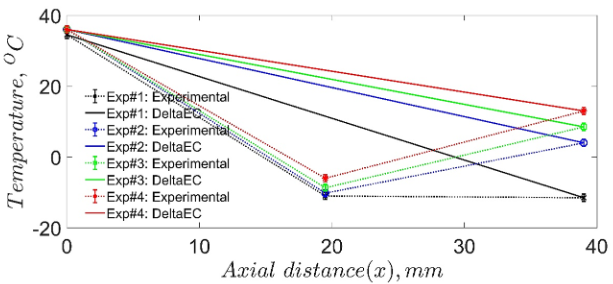
\includegraphics[width=.95\textwidth]{../fig/fig_Litterature/ATE_ProfilsAX_5mm.png}};}
		\caption{}
		\label{fig:ATE_ProfilsAX_5mm}
	\end{subfigure}		
	\begin{subfigure}{.47\textwidth}
		\centering
		\external{fig_ATE_ProfilsCHX_5mm}
%		\externalremake
		\tikz{\draw(0,0) node{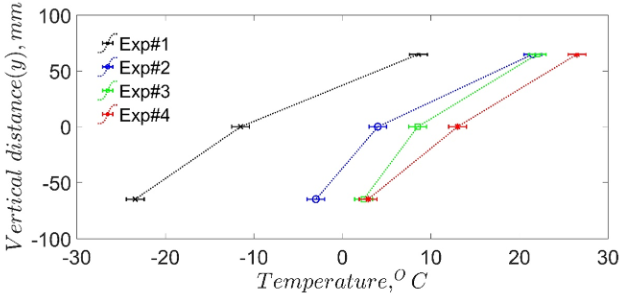
\includegraphics[width=.95\textwidth]{../fig/fig_Litterature/ATE_ProfilsCHX_5mm.png}};}
		\caption{}
		\label{fig:ATE_ProfilsCHX_5mm}
	\end{subfigure}	    
    \caption{Mesures et simulation linéaire de profils de température dans le régénérateur du \textsc{Tacot} pour différentes amplitudes acoustiques \cite{ramadan_design_2021}. \subref{fig:ATE_ProfilsAX_5mm} profils axiaux, et \subref{fig:ATE_ProfilsCHX_5mm}, profils transverses du côté de l'échangeur froid.}
    \label{fig:ATE_Profils_5mm}
\end{figure}

\subsection{Géométrie du réfrigérateur \textsc{Tacot}}
\subsubsection{Cavité thermoacoustique}
Le projet \textsc{Tacot} apporte beaucoup de contraintes pour la conception du réfrigérateur, et l'une des principales est la compacité. Contrairement aux autres systèmes thermoacoustiques existant et bien plus volumineux tels que le liquéfacteur de gaz naturel développé par Swift et Wollan au Los Alamos National Laboratory \cite{swift_thermoacoustics_2002, wollan_development_2002}, ou le réfrigérateur cryogénique thermoacoustique spatial (STAR) \cite{adeff_measurement_1991, garrett_thermoacoustic_1993}, les dimensions doivent être réduites tout en conservant un pompage de chaleur efficace. 

\begin{figure}[!ht]
    \centering
    \external{fig_SchemaGeneralTACOT}
%    \externalremake
    \begin{tikzpicture}[scale=.5]
	\node[anchor=south west, inner sep=0] (image) at (0,0) {\includegraphics[angle=0,origin=c,width=.6\textwidth]{../fig/fig_TACOTSchematics/TACOT.png}};
	
	\node[anchor=east, inner sep=0] (imagecropped) at (image.west) {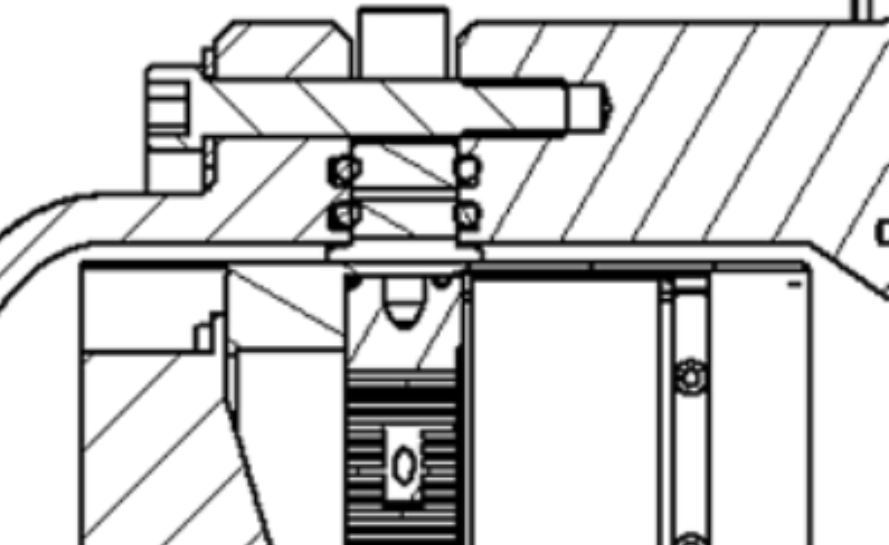
\includegraphics[angle=0,origin=c,width=.35\textwidth]{../fig/fig_TACOTSchematics/TACOT_Cropped.png}};

\draw[black, very thick, dashed, rounded corners] (imagecropped.north west) rectangle (imagecropped.south east);
%\draw[black, very thick, dashed, rounded corners] ($(AHX)+(-1.5cm,3cm)$) rectangle ($(CHX)+(.75cm,-.5cm)$);
	
	\begin{scope}[x={(image.south east)},y={(image.north west)}]
	
%		\filldraw (0,0) circle (2pt); 
%		\filldraw[green] (1,0) circle (1pt);
%		\filldraw[red] (1,1) circle (1pt);		
%		\filldraw[blue] (0,1) circle (1pt);
%		\draw[help lines,xstep=.1,ystep=.1] (0,0) grid (1,1);
%		\fill[orange, rounded corners, opacity=1,draw=orange] (.46,.65) -- ++(132:.09) -- ++(0,-.44) -- ++(48:.09) -- cycle;
		\draw[MatlabYellow,rounded corners,very thick,preaction={fill=MatlabYellow!20,opacity=.5}] (.46,.65) -- ++(132:.09) -- ++(-.03,0) -- ++(0,-.44) --++(.03,0) -- ++(48:.09) -- cycle; %node[left,pos=.5,label={[rotate=90]center:Cavité}]{};
		\draw[MatlabYellow] (.415,0.5) node [label={[rotate=90]center:\textbf{Cône}}]{};
		
%		\draw[blue] (.5,.5) node [anchor=center, preaction={fill=black!20,opacity=.7}] {RIX};
%		\draw[red] (.33,.5) node [anchor=center, preaction={fill=black!20,opacity=.7}] {TA core};	
	
		\draw[MatlabPurple,rounded corners,very thick,preaction={fill=MatlabPurple!20,opacity=.5}] (.365,.7) rectangle (.245,.3) node[pos=.5,label={[rotate=90]center:\textbf{Noyau}}]{};
		
		\node (AHX) at (.27,.65) {};
		\node (Reg) at (.32,.65) {};
		\node (CHX) at (.36,.65) {};
		\node (RIX) at (.77,.4) {};

		\node (HP) at (.19,.4) {};
		
		\draw[<-,very thick,MatlabOrange] (AHX.center) to[out=90,in=0] ($(AHX)+(-.2,.41)$) node[left]{\begin{tabular}{r} Echangeur de chaleur ambiant \\ (HXA) \end{tabular}};		
		\draw[<-,very thick] (Reg.center) to ($(Reg)+(0,.4)$) node[above]{Régénérateur};
		\draw[<-,very thick,MatlabBlue] (CHX.center) to[out=90,in=180] ($(CHX)+(.2,.41)$) node[right]{\begin{tabular}{l} Echangeur de chaleur froid \\ (HXF) \end{tabular}};
		
		\draw[->,very thick,green!50!black] ($(RIX)+(0,-.4)$) -- (RIX.center) node[pos=0,anchor=north]{\begin{tabular}{c}Source acoustique principale \\ (SA1) \end{tabular}};
		\draw[->,very thick,green!50!black] ($(HP)+(0,-.4)$) -- (HP.center) node (SA2) [pos=0,anchor=north]{\begin{tabular}{c}Source acoustique secondaire \\ (SA2) \end{tabular}};
		
%		\draw [white] (.455,.5) node{+};
%		\draw [white] (.41,.65) node{+};
%		\draw [white] (.41,.5) node{+};
%		\draw [white] (.41,.35) node{+};

		\draw[black, very thick, dashed, rounded corners] ($(AHX)+(-.14,.2)$) node(a){} rectangle ($(CHX)+(.07,-.1)$);
		
		\draw[black, very thick, dashed] (a) -- (imagecropped.north east);
		\draw[black, very thick, dashed] ($(a)+(0,-.3)$) -- (imagecropped.south east);
		

	\end{scope}
	
	\draw(imagecropped.south) node[below]{\small \textbf{(a)}};		
	\draw(SA2.south -| image.south) node{\small \textbf{(b)}};
	
\end{tikzpicture}
    \caption{Schéma général du réfrigérateur \textsc{Tacot} extrait de \cite{ramadan_design_2021}. \textbf{(a)} agrandissement sur la boucle de rétroaction entre le noyau et le bâti de la machine, et \textbf{(b)} ensemble de la machine. Le noyau thermoacoustique et le cône d'adaptation d'impédance sont mis en évidence.}
    \label{fig:SchemaGeneralTACOT}
\end{figure}

Pour cela, une géométrie coaxiale pour la cavité thermoacoustique est préférée à celle toroïdale usuellement utilisée en suivant les travaux de Poignand \textit{et al.} \cite{poignand_thermoacoustic_2011, poignand_analysis_2013}, et est présentée sur la figure~\ref{fig:SchemaGeneralTACOT}\textbf{(b)}. Dans ce cas, la boucle de rétroaction du guide d'onde se trouve tout autour du noyau placé au centre de la cavité thermoacoustique, ce que montre la figure~\ref{fig:SchemaGeneralTACOT}\textbf{(a)}.

L'ajout d'une source acoustique secondaire au voisinage du noyau permet également de gagner en compacité, en remplaçant un résonateur plus long par la masse de son équipage mobile et la souplesse de sa suspension, tel que réalisé dans les références \cite{poese_thermoacoustic_2004, poignand_thermoacoustic_2011, poignand_analysis_2013}. En plus de permettre une diminution du volume de la machine, utiliser une source secondaire offre plus de flexibilité qu'un résonateur sur la relation entre pression acoustique et vitesse particulaire, et facilite en particulier le ciblage du déphasage optimal entre pression et vitesse acoustiques au sein du noyau thermoacoustique \cite{poignand_thermoacoustic_2011, poignand_analysis_2013}.\smallskip

Par ailleurs, le mélange de gaz contient de l'hélium très volatile, et qui plus est, à haute pression. La conception de la machine doit donc prendre en compte cette difficulté et l'appliquer dans le choix des dimensions du bâti, des joints toriques, et bien entendu des nombreuses traversées qui joignent l'intérieur et l'extérieur de la cavité. La tenue en pression du mélange gazeux est affiché sur la figure~\ref{fig:TenuePressionStatique}. \echaf{on y voit que la durée avant vidange est blabla}.

\begin{figure}[!ht]
	\centering
	\external{fig_TenuePressionStatique}
	\externalremake
	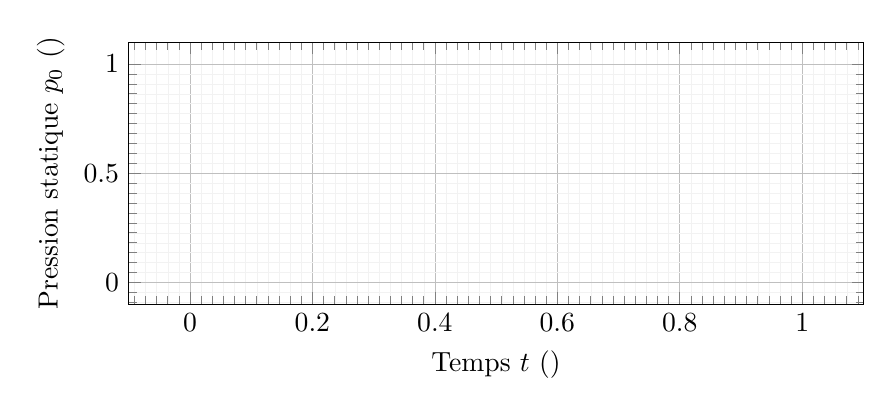
\begin{tikzpicture}
    \def\width{.9*\textwidth};
    \def\height{.45*\width};
    \def\spx{.25cm};
    \def\spy{1.25cm};
    \def\legx{.5cm};
    \def\legy{\legx};
    \def\prop{.45};

    
    \begin{axis}[name=TenuePress,width={\width},height={\height},
    grid=both, minor tick num=10, 
    grid style={line width=.1pt, draw=gray!10},
    major grid style={line width=.2pt,draw=gray!50},
    xlabel={Temps $t$ (\unit{\jour})},
    ylabel={Pression statique $p_0$ (\unit{\pascal})},
%    xmin=0,xmax=75,ymin=0,ymax=.5/1000,
%    xtick={0,25,50,75,100}, ytick={0,1e-4,...,10e-4},
    scaled y ticks = false,
    domain=0:100,
    legend cell align={left},
    legend style = {at={($(1,1)+(-2mm,-2mm)$)},anchor = north east,rounded corners}
    ]
    
%    \addplot[Plasma1, ultra thick] coordinates {(1,1),}

    \end{axis}
\end{tikzpicture}
%	\includegraphics[width=.7\textwidth]{example-image}
	\caption{Mesures de pression statique dans le réfrigérateur \textsc{Tacot} au cours du temps. \echaf{avec data du pc manip tacot}}
	\label{fig:TenuePressionStatique}
\end{figure}


\subsubsection{Noyau thermoacoustique}
Au c\oe{}ur de la machine qui le contient, le noyau est composé d'un régénérateur représenté sur la figure~\ref{fig:TacotPhotosNoyau_Regen} encadré par deux échangeurs de chaleur représentés sur les figures~\ref{fig:TacotPhotosNoyau_AHX} et \subref{fig:TacotPhotosNoyau_CHX}. Le premier est l'échangeur ambiant et a pour rôle d'extraire la chaleur qui s'accumule de ce côté du noyau, afin d'éviter l'échauffement global de la machine. Le second est l'échangeur froid, et sa fonction et de simuler une charge thermique à refroidir. 

\begin{figure}[!ht]
    \centering
	\begin{subfigure}{.32\textwidth}
		\centering
		\external{fig_TacotPhotosNoyau_AHX}
%		\externalremake
		\tikz{\draw(0,0) node{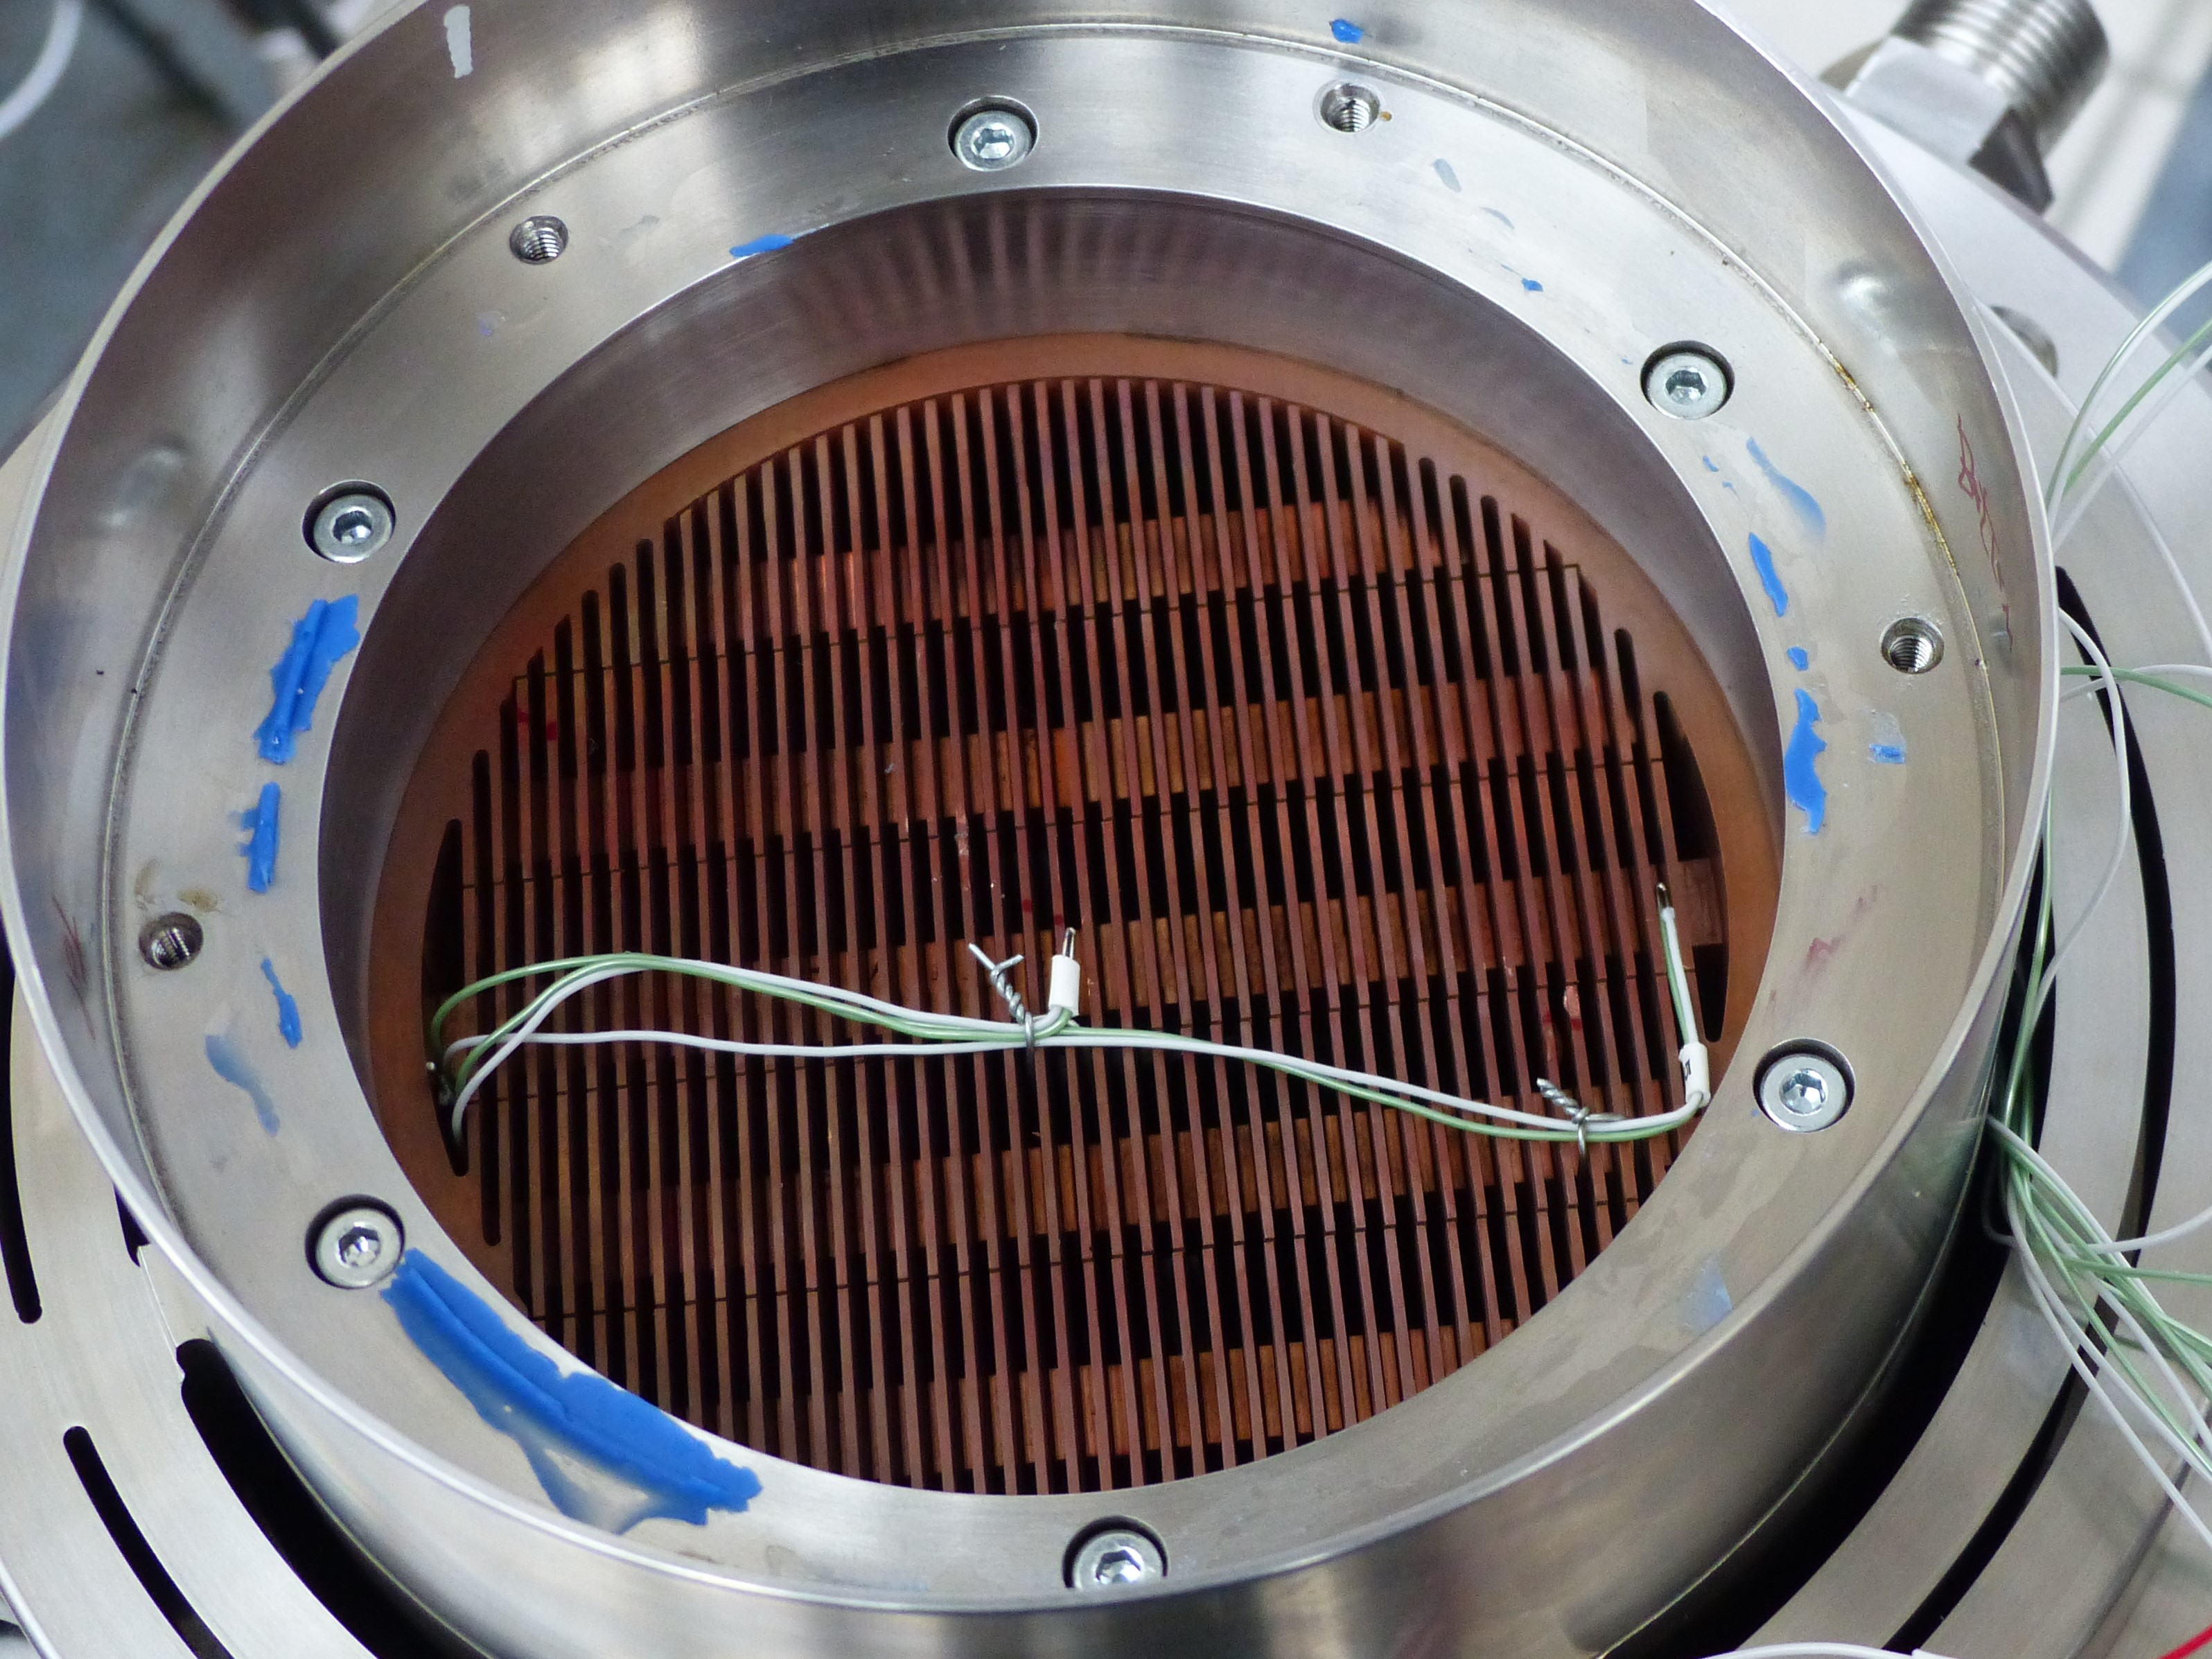
\includegraphics[width=.95\textwidth]{../fig/fig_TacotPhotos/AHX.JPG}};}
		\caption{}
		\label{fig:TacotPhotosNoyau_AHX}
	\end{subfigure}		
	\begin{subfigure}{.32\textwidth}
		\centering
		\external{fig_TacotPhotosNoyau_Regenerateur}
%		\externalremake
		\tikz{\draw(0,0) node{\includegraphics[width=.95\textwidth]{../fig/fig_TacotPhotos/Regenerateur.JPG}};}
		\caption{}
		\label{fig:TacotPhotosNoyau_Regen}
	\end{subfigure}	
	\begin{subfigure}{.32\textwidth}
		\centering
		\external{fig_TacotPhotosNoyau_CHX}
%		\externalremake
		\tikz{\draw(0,0) node{\includegraphics[width=.95\textwidth]{../fig/fig_TacotPhotos/CHX.JPG}};}
		\caption{}
		\label{fig:TacotPhotosNoyau_CHX}
	\end{subfigure}	    
    \caption{Composition du noyau thermoacoustique : \subref{fig:TacotPhotosNoyau_AHX} \'Echangeur ambiant, \subref{fig:TacotPhotosNoyau_Regen} régénérateur, et \subref{fig:TacotPhotosNoyau_CHX} échangeur froid.}
    \label{fig:TacotPhotosNoyau}
\end{figure}

Ces trois éléments sont ensuite insérés dans un tube cylindrique qui se fixe sur le bâti de la machine pour maintenir l'espace nécessaire à la boucle de rétroaction acoustique, ce que montre la figure~\ref{fig:PhotoSchemaNoyau}.

\begin{figure}[!ht]
    \centering
	\begin{subfigure}[c]{.49\textwidth}
		\centering
		\external{fig_PhotoNoyau}
%		\externalremake
    \tikz{\draw(0,0) node{\includegraphics[width=.97\textwidth]{../fig/fig_TacotPhotos/NoyauMonte.JPG}};}
		\caption{}
		\label{fig:PhotoNoyau}
	\end{subfigure}		
	\begin{subfigure}[c]{.49\textwidth}
		\centering
		\external{fig_SchemaNoyau}
%		\externalremake
		\begin{tikzpicture}[scale=.2]
	\def\rCHX{14cm};
	\def\lCHX{.7cm};
	\def\rREG{14.8cm};
	\def\lREG{3.9cm};
	\def\rAHX{11cm};
	\def\lAHX{2.3cm};
	\def\rRIX{10.8cm};
	\def\rCONE{16.4cm};
	
	
	\fill[pattern=horizontal lines,pattern color=MatlabOrange,draw=black] (0,-\rAHX) rectangle ++(\lAHX,2*\rAHX);
	\draw[MatlabOrange] (\lAHX/2,-\rCHX) node(AHX)[below=1cm, anchor=north east]{\'Echangeur ambiant};

	\filldraw[draw=black,fill=gray!50!white] (0,\rAHX) rectangle (\lAHX,\rREG);		% côtés où l'eau circule
	\filldraw[draw=black,fill=gray!50!white] (0,-\rAHX) rectangle (\lAHX,-\rREG);	%
	
	\draw[MatlabOrange,->] (AHX.north east) to[out=90,in=-90] (\lAHX/2,-\rAHX);
	
	\begin{scope}[xshift=\lAHX] % Reg
		\fill[pattern=crosshatch,pattern color=gray,draw=black] (0,-\rREG) rectangle ++(\lREG,2*\rREG);
		\draw[black] (\lREG/2,0) node[anchor=center, rounded corners, rotate=90, fill=white, fill opacity=.5, text opacity=1]{Régénerateur};
	\end{scope}
	
	\begin{scope}[xshift=\lAHX+\lREG] % CHX
		\fill[pattern=horizontal lines,pattern color=MatlabBlue,draw=black] (0,-\rCHX) rectangle ++(\lCHX,2*\rCHX);
		\draw[MatlabBlue] (\lCHX/2,-\rCHX) node(CHX)[below=1cm,anchor=north west]{\'Echangeur froid};

				
	\filldraw[draw=black,fill=gray!50!white] (0,\rREG) rectangle (\lCHX,\rCHX);		% côtés où l'eau circule
	\filldraw[draw=black,fill=gray!50!white] (0,-\rREG) rectangle (\lCHX,-\rCHX);	%
	
	\draw[MatlabYellow,rounded corners,very thick] (\lCHX,-\rCONE) -- ++(\lAHX,0) -- ++(2*\lAHX,{\rCONE-\rRIX}) -- ++(0,2*\rRIX) node(Cone){} -- ++(-2*\lAHX,{\rCONE-\rRIX})  -- ++(-\lAHX,0) -- cycle;
	
	\draw[MatlabBlue,->] (CHX.north west) to[out=90,in=-90] (\lCHX/2,-\rCHX);
%	\draw[MatlabYellow,->] ($(Cone.center)+(3*\lAHX,3*\lAHX)$) node[anchor=south]{Cone d'adaptation d'impédance} to[out=-90,in=0] (Cone);
	\end{scope}
	
	\draw[MatlabPurple,rounded corners,very thick] (0,-\rCONE) rectangle ++({\lAHX+\lREG+\lCHX},2*\rCONE);
	
%	\draw[green!50!black] (0,0) node[left]{\begin{tabular}{r}Source \\ acoustique \\ secondaire \end{tabular}};
%	\draw[green!50!black] ({\lCHX+\lREG+4*\lAHX},0) node[right]{\begin{tabular}{l} Source \\ acoustique \\ principale\end{tabular}};
	 
	  \draw[<-, dashed] ({-(\lAHX+\lREG+\lCHX)/2},{\rCONE+\lAHX}) node[left]{$\mathbf e_x$} -- ({(\lAHX+\lREG+\lCHX)*1.5},{\rCONE+\lAHX});
	  \draw[|-] (0,{\rCONE+\lAHX}) -- ++(\lAHX,0) node[midway,above=1pt, text=MatlabOrange]{\num{2.3}};
	  \draw[|-] (\lAHX,{\rCONE+\lAHX}) -- ++(\lREG,0) node[midway,above=8pt]{\num{3.9}};
	  \draw[|-|] ({\lAHX+\lREG},{\rCONE+\lAHX}) -- ++(\lCHX,0) node[midway,above=1pt, text=MatlabBlue]{\num{.7}};
	  
	  \draw[->, dashed] (-\lAHX,-1.1*\rCONE) -- ++(0,{2.2*\rCONE+\lAHX}) node[above]{$\mathbf e_r$};
	  \draw[|-|] (-\lAHX,0) node[left]{\num{0}} -- (-\lAHX,\rAHX) node[left, text=MatlabOrange]{\num{5.5}};
	  \draw[-|] (-\lAHX,0) -- (-\lAHX,\rREG) node[left]{\num{7.4}};
	  \draw[-|] (-\lAHX,0) -- (-\lAHX,\rCHX) node[below left, text=MatlabBlue]{\num{7}};
	  
	
\end{tikzpicture}
		\caption{}
		\label{fig:SchemaNoyau}
	\end{subfigure}	    
    \caption{Noyau thermoacoustique assemblé. \subref{fig:PhotoNoyau} photographie de l'assemblage, \subref{fig:SchemaNoyau} schéma agrandi des zones violette et jaune de la figure~\ref{fig:SchemaGeneralTACOT}. Les dimensions sont données en \unit{\centi\meter}.}
    \label{fig:PhotoSchemaNoyau}
\end{figure}


Les axes $\mathbf e_x$ et $\mathbf e_r$ sont alors respectivement associés aux directions axiale et radiale du noyau, respectivement avec pour sens positif choisi le sens de l'échangeur froid vers l'échangeur ambiant pour le premier, et du centre du noyau vers l'extérieur pour le second. Un repère $(O;\mathbf e_{x,0},\mathbf e_{y,0},\mathbf e_{z,0})$ est également défini sur la figure~\ref{fig:BancEssaisComplet} pour évaluer l'orientation du réfrigérateur dans la suite de ce manuscrit.\medskip

\paragraph{Régénérateur} Le régénérateur utilisé dans le \textsc{Tacot} est composé de \echaf{combien} disques de tissus métalliques (Gantois, modèle : 102045) empilés dans une enceinte cylindrique de diamètre intérieur $D_{\sf reg}=\qty{148}{\mm}$ et de longueur $L_{\sf reg}=\qty{39}{\mm}$ pour atteindre une porosité $\Phi=\qty{68}{\percent}$. Cette porosité est définie par la relation

\begin{align}
	\Phi &= \frac{V_{\sf gaz}}{V_{\sf tot}}, \label{eq:Porosite_Volume}%\\
%		 &= \frac{V_{\sf tot}-V_{\sf metal}}{V_{\sf tot}} \nonumber\\
%		 &= 1 - \frac{m_{\sf metal}}{m_{\sf tot}} \label{eq:Porosite_Masse}
\end{align}
où $V_{\sf gaz}$ représente le volume occupé par le gaz dans le régénérateur, et $V_{\sf tot}$ le volume total du régénérateur. Il est à noter que ce régénérateur est différent de celui utilisé dans l'article de Ramadan \textit{et al.}~\cite{ramadan_design_2021}, car le but est de comparer les performances et le comportement du réfrigérateur dans le cas où la porosité du noyau est modifiée. 

La masse de tissus $m_{\sf tissus}$ à utiliser pour atteindre la porosité souhaitée est déduite de l'équation \eqref{eq:Porosite_Volume} et s'écrit 

\begin{align}
%		 &= \frac{V_{\sf tot}-V_{\sf tissus}}{V_{\sf tot}} \nonumber\\
%	\Phi &= 1 - \frac{m_{\sf tissus}}{m_{\sf tot}}. \label{eq:Porosite_Masse} \\
	m_{\sf tissus} &= (1-\Phi) m_{\sf tot}, \label{eq:MasseTissus_Porosite}
\end{align}
où $m_{\sf tot}$ représente la masse d'un cylindre de mêmes dimensions que le régénérateur, intégralement constitué du même acier inoxydable que les tissus, soit de l'acier inoxydable 316L.

Le milieu ainsi constitué est poreux et tortueux car l'orientation des disques de tissus est aléatoire, et le rayon hydraulique est défini par  %\echaf{ajouter source pour justifier que les matériaux type "mousse" se comporte comme du cylindrique : UPDATE dans Swift TA unifying... chapitre 7 (tortuous porous media)}

\begin{equation}
	r_h = d_w\frac{\Phi}{4(1-\Phi)},
	\label{eq:DefRayonHydrauGantois}
\end{equation}
avec $d_w$ le diamètre du fil \cite{swift_thermoacoustics_2017}. Ce milieu poreux dispose d'une certaine capacité à laisser passer un écoulement. C'est la perméabilité notée $\mathbf K_p$, qui intervient dans la loi de Darcy

\begin{equation}
%	\mathbf K_p = \echaf{v_{\sf ref}\frac{\nu \Delta x}{\Delta P}},
	\mathbf u_{\sf ref} = -\frac{\mathbf K_p}{\mu} (\nabla p - \rho_0 \mathbf g),
	\label{eq:DefPermeabilite_Wikipedia}
\end{equation}
où $\mathbf u_{\sf ref}$ est le débit de filtration d'un fluide qui s'écoule dans le milieu poreux et causé par un gradient de pression $\nicefrac{\Delta P}{\Delta x}$ \cite{nield_convection_2013, dullien_porous_1992}. La perméabilité ne dépend par ailleurs que du milieu, et il existe dans la littérature des formulations de la perméabilité ne prenant en compte que la géométrie interne \cite{dullien_porous_1992}. En faisant l'hypothèse d'un milieu constitué d'un matériau isotrope, la formulation retenue s'écrit

\begin{equation}
	K_p = \echaf{\frac{4 r_h^2 \Phi}{8}},
	\label{eq:DefPermeabilite_LISN}
\end{equation}
et donne des résultats satisfaisants pour le développement de modèles \cite{hireche_experimental_2020, baltean_gravity_2025}.\smallskip

\echaf{Toutefois, la définition de la perméabilité dans l'équation de Darcy considère un écoulement unidirectionnel, stationnaire et suffisamment lent \cite{dullien_porous_1992}. De plus, l'empillement de tissus crée un milieu multicouche qui n'est certainement pas isotrope, Ce qui nécessite de considérer le caractère tensoriel de cette quantité.\echaf{ vraiment utile de rentrer dans les détails d'un modèle multi couche de la permeabilité ? }\cite{tan_new_2024}}\medskip

À l'intérieur de ce matériau poreux, le champ acoustique est primordial et requiert le respect de plusieurs conditions. Tout d'abord, le contact thermique doit être le meilleur possible afin de garantir une égalité des températures du fluide et du solide poreux pour toute position dans le régénérateur. Cela implique que le rayon hydraulique des pores soit largement inférieur à l'épaisseur de chacune des couches limites thermique et visqueuse, ce qui s'écrit
\begin{equation}
	\frac{\delta_{\kappa,\nu}}{r_h} \gg 1.
	\label{eq:ConditionIso_dkdv}
\end{equation}

Pour le fluide considéré, les épaisseurs de couches limites sont tracées en fonction de la fréquence sur la figure~\ref{fig:dKdV}, ce qui permet de montrer l'écart d'un ordre de grandeur avec le rayon hydraulique du des pores du régénérateur.

\begin{figure}[!ht]
    \centering
    \external{fig_dKdV}
%    \externalremake
    \begin{tikzpicture}
    \def\width{.9*\textwidth};
    \def\height{.45*\width};
    \def\spx{.25cm};
    \def\spy{1.25cm};
    \def\legx{.5cm};
    \def\legy{\legx};
    \def\prop{.45};
    \def\xcursor{47};
    \def\ycursorV{9.112e-5};
    \def\ycursorK{1.4452e-4};
    \def\rh{2.81e-5};
    
    \begin{axis}[name=dKdV,width={\width},height={\height},
    grid=both, minor tick num=10, 
    grid style={line width=.1pt, draw=gray!10},
    major grid style={line width=.2pt,draw=gray!50},
    xlabel={Fréquence $f$ [\unit{\Hz}]},
    ylabel={\'Epaisseurs de couches limites $\delta_{\kappa,\nu}$ [\unit{\m}]},
    xmin=0,xmax=75,ymin=0,ymax=.5/1000,
    xtick={0,25,50,75,100},
    extra x ticks={47},
    extra x tick style={
        grid=major,
        xticklabel={\num{47}},
        xticklabel style={yshift=0, anchor=north}
        },
    extra y ticks={\rh},
    extra y tick style={
        grid=major,
        yticklabel={$r_h$},
        yticklabel style={yshift=1mm, anchor=east}
        },
    ytick={0,1e-4,...,10e-4},
%    ytick={0,2.81/100000,9.1120/100000,1.4452/10000,
%    	2.5/10000,5/10000,1/1000},
    scaled y ticks = false,
    domain=0:100,
    legend cell align={left},
    legend style = {at={($(1,1)+(-2mm,-2mm)$)},anchor = north east,rounded corners}
    ]
        \addplot[solid,ultra thick,draw=Plasma1] file {../fig/fig_dKdV/data/data_dK.txt};
        \addplot[solid,ultra thick,draw=Plasma64] file {../fig/fig_dKdV/data/data_dV.txt};
        \filldraw[Plasma1] (\xcursor,\ycursorK) circle (2pt) node[above right]{$\delta_\kappa=\qty{\ycursorK}{\meter}$};
        \filldraw[Plasma64] (\xcursor,\ycursorV) circle (2pt) node[below left]{$\delta_\nu=\qty{\ycursorV}{\meter}$};
%        \draw[dashed,black!50] (\xcursor,0) -- (\xcursor,\ycursorK);
%        \draw[dashed,Plasma33] (\xcursor,\ycursorK) -- (0,\ycursorK) node[left]{\num{1.4452e-4}};
%        \draw[dashed,Plasma66] (\xcursor,\ycursorV) -- (0,\ycursorV) node[left]{\num{9.1120e-5}};
%         \draw[dashed,black!50] ({axis cs:\xcursor,0}|-{rel axis cs:0,0}) -- ({axis cs:\xcursor,0}|-{rel axis cs:0,\ycursorK});
       \addplot[loosely dashed,draw=black, ultra thick] {\rh};
       \draw(0,\rh) node[above right]{\qty{\rh}{\meter}};
        
        \legend{$\delta_\kappa$ \\ $\delta_\nu$ \\ $r_h$ \\};
    \end{axis}
\end{tikzpicture}
    \caption{\'Evolution des épaisseurs de couches limites thermique $\delta_\kappa$ et visqueuse $\delta_\nu$ en fonction de la fréquence, définies par le système d'équations~\eqref{eq:CouchesLimites}. Elles sont comparées au rayon hydraulique $r_h$.}
    \label{fig:dKdV}
\end{figure}

Ce cycle où les transformations sont isothermes est celui de Stirling, pour lequel les oscillations de pression et de vitesse sont en phase. Cependant, ce cycle représente un comportement asymptotique prenant place dans une machine thermoacoustique, tout comme le cycle de Brayton. Dans la réalité, il a été montré dans la littérature portant sur les machines à plusieurs sources qu'il existe une vitesse acoustique optimale pour une pression acoustique donnée~\cite{poignand_analysis_2013, poignand_etude_2006, poignand_optimal_2007, poignand_thermoacoustic_2011}. \echaf{Les puissances thermiques pompées et le gradient de températures le long du régénérateur sont les plus élevées lorsque la vitesse acoustique atteint une amplitude donnée par}

\begin{subequations}
	\begin{align}
		|v|_{\sf opt} &= \sqrt{\frac{4 \omega (kh+k_se_s) \left(1-\Prandtl^2\right)\left(1-\frac{\delta_\nu}{h}+\frac{\delta_\nu^2}{2h^2}\right)}{\delta_\kappa \rho_0 C_p \left(1-\Prandtl\sqrt{\Prandtl}\right)}}, & 	\label{eq:u_mag_opt_Gaelle}\\
		\intertext{et un déphasage écrit}
		\angle v_{\sf opt} &= \arctan\left[-\frac{1+\sqrt{\Prandtl}-\frac{\delta_\nu}{h}}{1-\big(1-\frac{\delta_\nu}{h} \big)\sqrt{\Prandtl}}\right]+n \pi, & n \in \mathbb{Z}.	\label{eq:u_arg_opt_Gaelle}
	\end{align}
	\label{eq:u_opt_Gaelle}
\end{subequations}
%\echaf{Remplacer $kh+k_s e_s$ par $\Phi k + (1-\Phi)k_s k_{s,frac}$ ? $\frac{\delta_\nu}{h}$ par $\frac{\delta_\nu}{r_h}$ ? -> redériver pour régénérateur}

Pour un régénérateur dans lequel les processus sont isothermes, ces équations sont modifiées et s'écrivent \echaf{détailler}

\begin{subequations}
	\begin{align}
		|v|_{\sf opt} &= \sqrt{\frac{2 \omega k_s(1-\Phi)}{\rho_0 C_p \IM[g_D]}},\label{eq:u_mag_opt_reg_Gaelle} \\
		\intertext{et}
		\angle v_{\sf opt} &= \arctan\left[-\frac{\IM[g]}{\RE[g]}\right],
	\end{align}
\end{subequations}
avec $g_D = \frac{f_\kappa + \Prandtl f_\nu^*}{(1-\Prandtl^2)|1-f_\nu^*|^2}$ et $g = \frac{f_\kappa-f_\nu^*}{(1+\Prandtl)(1-f_\nu^*)}$.

\begin{figure}[!ht]
    \centering
	\begin{subfigure}{.47\textwidth}
		\centering
		\external{fig_DeltaEC_u_opt_COP}
%		\externalremake
		\begin{tikzpicture}
    \def\width{.4*\textwidth};
    \def\height{\width};
    \def\spx{.25cm};
    \def\spy{1.25cm};
    \def\legx{.5cm};
    \def\legy{\legx};
    \def\prop{.45};
 
    
    \begin{axis}[width={\width},height={\height},
    view={0}{90},	
    colorbar,
%    grid=both, minor tick num=10, 
%    grid style={line width=.1pt, draw=gray!10},
%    major grid style={line width=.2pt,draw=gray!50},
    xlabel={Amplitude du débit $|u|_{\sf opt}$ (\unit{\cubic\meter\per\second})},
    ylabel={Phase du débit $\angle u_{\sf opt}$ (\unit{\degree})},
%    xmin=0,xmax=75,ymin=0,ymax=.5/1000,
%    xtick={0,25,50,75,100},
%    ytick={0,1e-4,...,10e-4},
%    ytick={0,2.81/100000,9.1120/100000,1.4452/10000,
%    	2.5/10000,5/10000,1/1000},
    scaled y ticks = false,
%    domain=0:100,
    legend cell align={left},
    legend style = {at={($(1,1)+(-2mm,-2mm)$)},anchor = north east,rounded corners}
    ]
    	\addplot3[surf, mesh/rows=21, shader=interp, patch type=bilinear] file {../fig/fig_DeltaEC_u_opt/data/data_DeltaEC_u_opt_COP.txt}; 
    \end{axis}
\end{tikzpicture}
		\caption{}
		\label{fig:DeltaEC_u_opt_COP}
	\end{subfigure}
	\begin{subfigure}{.47\textwidth}
		\centering
		\external{fig_DeltaEC_u_opt_DeltaT}
%		\externalremake
		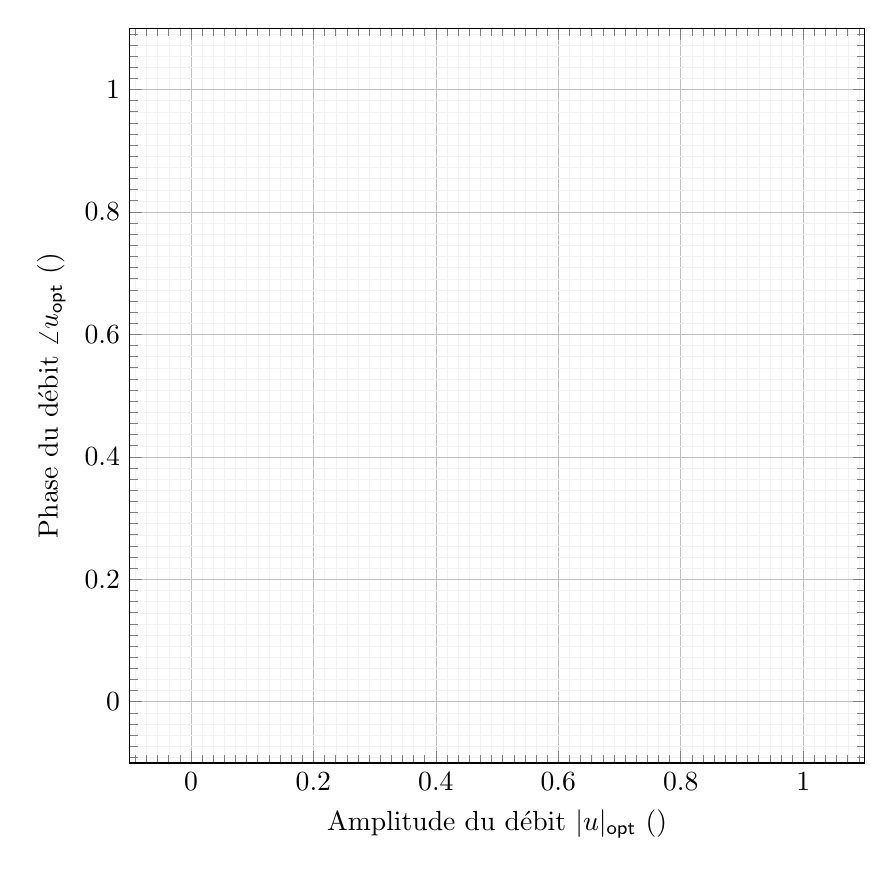
\begin{tikzpicture}
    \def\width{.9*\textwidth};
    \def\height{\width};
    \def\spx{.25cm};
    \def\spy{1.25cm};
    \def\legx{.5cm};
    \def\legy{\legx};
    \def\prop{.45};
 
    
    \begin{axis}[width={\width},height={\height},
    grid=both, minor tick num=10, 
    grid style={line width=.1pt, draw=gray!10},
    major grid style={line width=.2pt,draw=gray!50},
    xlabel={Amplitude du débit $|u|_{\sf opt}$ (\unit{\cubic\meter\per\second})},
    ylabel={Phase du débit $\angle u_{\sf opt}$ (\unit{\cubic\meter\per\second})},
%    xmin=0,xmax=75,ymin=0,ymax=.5/1000,
%    xtick={0,25,50,75,100},
%    ytick={0,1e-4,...,10e-4},
%    ytick={0,2.81/100000,9.1120/100000,1.4452/10000,
%    	2.5/10000,5/10000,1/1000},
    scaled y ticks = false,
    domain=0:100,
    legend cell align={left},
    legend style = {at={($(1,1)+(-2mm,-2mm)$)},anchor = north east,rounded corners}
    ]
        
    \end{axis}
\end{tikzpicture}
		\caption{}
		\label{fig:DeltaEC_u_opt_DeltaT}
	\end{subfigure}
	\begin{subfigure}{.47\textwidth}
		\centering
		\external{fig_DeltaEC_u_opt_Qth}
%		\externalremake
		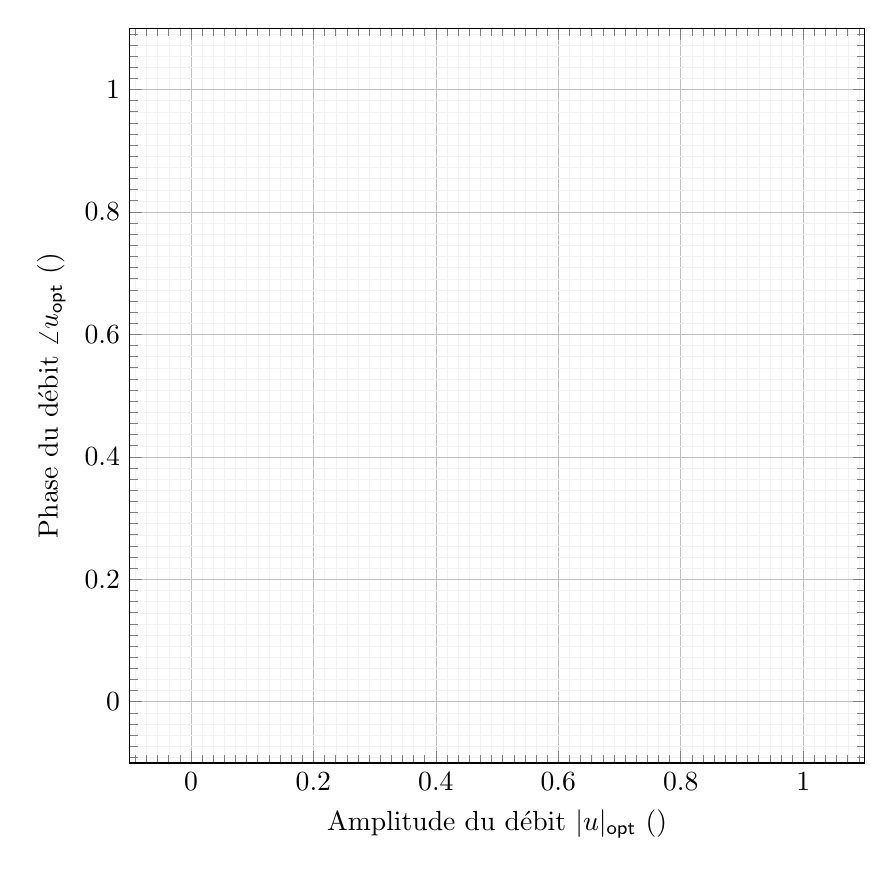
\begin{tikzpicture}
    \def\width{.9*\textwidth};
    \def\height{\width};
    \def\spx{.25cm};
    \def\spy{1.25cm};
    \def\legx{.5cm};
    \def\legy{\legx};
    \def\prop{.45};
 
    
    \begin{axis}[width={\width},height={\height},
    grid=both, minor tick num=10, 
    grid style={line width=.1pt, draw=gray!10},
    major grid style={line width=.2pt,draw=gray!50},
    xlabel={Amplitude du débit $|u|_{\sf opt}$ (\unit{\cubic\meter\per\second})},
    ylabel={Phase du débit $\angle u_{\sf opt}$ (\unit{\cubic\meter\per\second})},
%    xmin=0,xmax=75,ymin=0,ymax=.5/1000,
%    xtick={0,25,50,75,100},
%    ytick={0,1e-4,...,10e-4},
%    ytick={0,2.81/100000,9.1120/100000,1.4452/10000,
%    	2.5/10000,5/10000,1/1000},
    scaled y ticks = false,
    domain=0:100,
    legend cell align={left},
    legend style = {at={($(1,1)+(-2mm,-2mm)$)},anchor = north east,rounded corners}
    ]
        
    \end{axis}
\end{tikzpicture}
		\caption{}
		\label{fig:DeltaEC_u_opt_Qth}
	\end{subfigure}  
    \caption{Valeurs en fonction de l'amplitude et la phase du débit acoustique \ref{fig:DeltaEC_u_opt_COP} du coefficient de performance, \ref{fig:DeltaEC_u_opt_DeltaT} de l'écart de température de part et d'autre du régénérateur, et \ref{fig:DeltaEC_u_opt_Qth} du flux de chaleur thermoacoustique.}
    \label{fig:DeltaEC_u_opt}
\end{figure}

Au final, les dimensions du régénérateur sont résumés dans le tableau~\ref{tab:GeometrieTAC}, et les paramètres du fluides pour les points de fonctionnement du \textsc{Tacot}, dans le tableau~\ref{tab:ParamHydrauTAC}.

\begin{table}[!ht]
	\caption{Géométrie du noyau thermoacoustique.}
    \label{tab:GeometrieTAC}
    \centering
    \begin{tabular}{l@{\hspace{1cm}}l}
    	\hline
    	\textbf{Paramètre} & \textbf{Valeur} \\\hline\hline
    	Diamètre de l'échangeur ambiant $D_{\sf HXA}$ & \qty{110e-3}{\meter} \\
    	Longueur du l'échangeur ambiant $L_{\sf HXA}$ & \qty{23e-3}{\meter} \\
    	Diamètre du régénérateur $D_{\sf reg}$ & \qty{148e-3}{\meter} \\
    	Longueur du régénérateur $L_{\sf reg}$ & \qty{39e-3}{\meter} \\
    	Diamètre du l'échangeur froid $D_{\sf HXF}$ & \qty{140e-3}{\meter} \\
    	Longueur du l'échangeur froid $L_{\sf HXF}$ & \qty{7e-3}{\meter} \\
    	Diamètre du fil $d_w$ & \qty{53e-6}{\meter} \\
        Porosité du noyau $\Phi$ & \qty{68}{\percent} \\
        \hline
    \end{tabular}
\end{table}

\begin{table}[!ht]
    \caption{Paramètres thermiques et hydrauliques des expériences.}
    \label{tab:ParamHydrauTAC}
    \centering
    \begin{tabular}{l@{\hspace{1cm}}l}
    	\hline
    	\textbf{Paramètre} & \textbf{Valeur} \\\hline\hline
    	Fréquence d'opération $f_1$ & \qty{47}{\hertz} \\
    	Pression statique $p_0$ & \qty{4e6}{\pascal} \\
    	Rayon hydraulique $r_h$ & \qty{2.81e-5}{\meter}\\
    	Masse volumique $\rho_0$ & \qty{22.2}{\kilo\gram\per\cubic\meter} \\
        Célérité du son $c_0$ & \qty{547}{\meter\per\second} \\
        Capacité thermique isobare $C_p$ & \qty{1405}{\joule\per\kilo\gram\per\kelvin} \\
        Conductivité thermique du gaz $k_g$ & \qty{8.6e-2}{\watt\per\meter\per\kelvin} \\
        Couche limite thermique $\delta_\kappa$ & \qty{1.4452e-4}{\meter} \\
        Viscosité dynamique $\mu$ & \qty{2.4e-5}{\kilo\gram\per\meter\per\second} \\
        Couche limite visqueuse $\delta_\nu$ & \qty{9.1120e-5}{\meter} \\
        Perméabilité $K_p$ & \qty{2.68e-10}{\meter\squared} \\
       	Amplitude du débit acoustique optimal $|u|_{\sf opt}$ & \echaf{valeur} \\
		Phase du débit acoustique optimal $\angle u_{\sf opt}$ & \echaf{valeur} \\
        \hline
    \end{tabular}
\end{table}

\paragraph{\'Echangeurs de chaleur}

\begin{figure}[!ht]
    \centering
	\begin{subfigure}[c]{.47\textwidth}
		\centering
		\external{fig_AHXSchema}
%    	\externalremake
	    \tikz{\draw (0,0) node {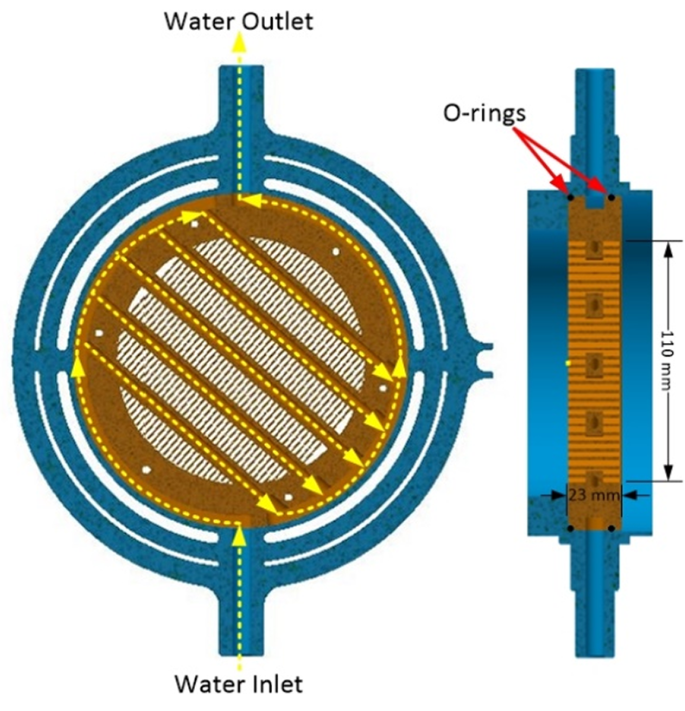
\includegraphics[width=.95\textwidth]{../fig/fig_AHXfromATE/AHXfromATE.png}};}
		\caption{}
		\label{fig:AHXschema}
	\end{subfigure}		
	\begin{subfigure}[c]{.47\textwidth}
		\centering
		\external{fig_CHXSchema}
%		\externalremake
		\tikz{\draw(0,0) node{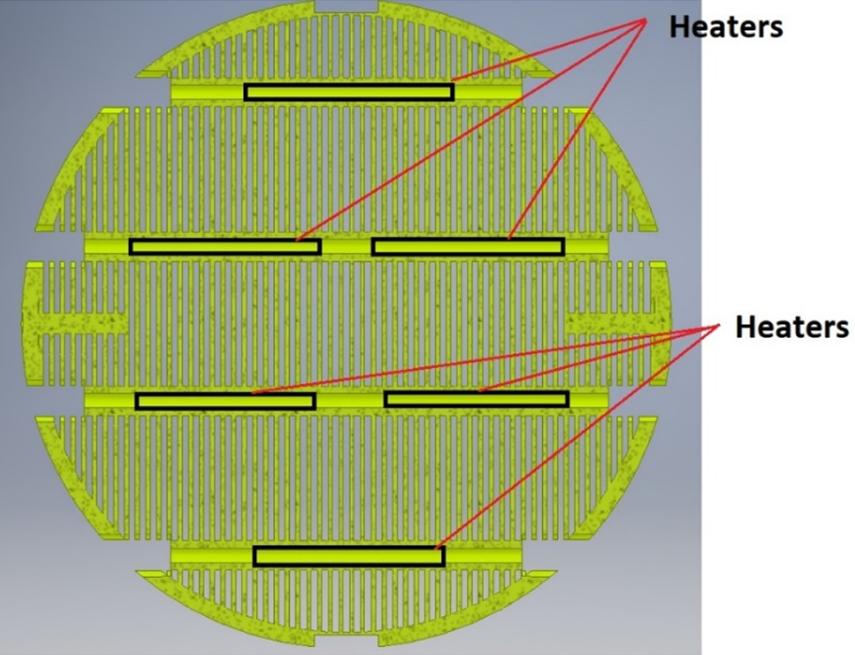
\includegraphics[width=.95\textwidth]{../fig/fig_CHXfromATE/SchemaCHX.png}};}
		\caption{}
		\label{fig:CHXschema}
	\end{subfigure}	    
    \caption{Schémas des échangeurs \cite{ramadan_design_2021}. \subref{fig:AHXschema} échangeur ambiant, où les trait pointillés jaune montrent le circuit d'eau, et \subref{fig:CHXschema} échangeur froid sur lequel l'emplacement des cartouches chauffantes est indiqué par les rectangles. \echaf{mettre version vierge du CHX}}
    \label{fig:HXschema}
\end{figure}

Le pompage de chaleur par effet thermoacoustique est exploité par des échangeurs conçus en même temps que le reste du dispositif expérimental, en utilisant le logiciel \textsc{DeltaEC} pour déterminer les caractéristiques comme la longueur axiale, la surface, ou la porosité. Concernant cette dernière, il faut faire en sorte de laisser s'écouler librement le fluide sans causer de pertes de charges trop importantes, tout en conservant une grande surface de contact. Par ailleurs, leurs longueurs sont au moins deux fois supérieures à l'excursion particulaire crête à crête, qui est de l'ordre de \qty{1}{\centi\meter} dans les conditions d'opération de la machine. Cependant, les paramètres calculés avec \textsc{DeltaEC} ne sont pas suffisant pour concevoir un échangeur fonctionnel, et le fonctionnement de chacun de ces échangeur étant radicalement différent l'un de l'autre, quelques détails de conception propres à chacun sont à présenter.

\subparagraph{\'Echangeur ambiant} 
De l'énergie mécanique est continuellement apportée au système par les sources acoustiques, ce qui s'accompagne du pompage thermoacoustique de l'extrémité froide à l'extrémité chaude du noyau. Pour fixer la température de ce côté à une température ambiante et éviter l'échauffement global de la machine, l'échangeur ambiant extrait un flux de chaleur $\dot Q_a$ au fluide chaud pour la céder à de l'eau froide qui circule à l'intérieur en suivant la relation 

\begin{equation}
	\dot Q_a = \dot m C_p \Delta T.
	\label{eq:Qa_Definition}
\end{equation}

Pour dimensionner l'échangeur, une méthode combinant un modèle \textsc{DeltaEC} et une analyse basée sur la différence de température logarithmique moyenne est utilisée pour déterminer la longueur, le diamètre et la porosité de l'échangeur, de même que l'architecture nécessaire au bon échange de chaleur, comme par exemple le nombre d'ailettes, leur épaisseur et leur espacement, et les diamètres des conduits d'eau \cite{ramadan_design_2021}. \smallskip

L'architecture proposée pour l'échangeur est représentée sur la figure~\ref{fig:AHXschema}. Elle comporte cinq canaux centraux qui divisent le flux d'eau total pour le faire circuler sur toute la section de l'échangeur. L'apport et l'évacuation de l'eau se font par deux conduits périphériques, connectés de sorte à faire suivre le chemin tracé en pointillées jaunes sur la figure. Les canaux centraux sont entourés de \num{190} ailettes dont l'épaisseur vaut \qty{1}{\milli\meter}, et qui sont séparées l'une de l'autre par \qty{1.5}{\milli\metre}. La porosité ainsi obtenue est donc de \qty{32}{\percent} \echaf{valeur à vérifier}.

\begin{figure}[!ht]
	\centering
	\external{fig_TemperatureAHX_InOut}
%	\externalremake
	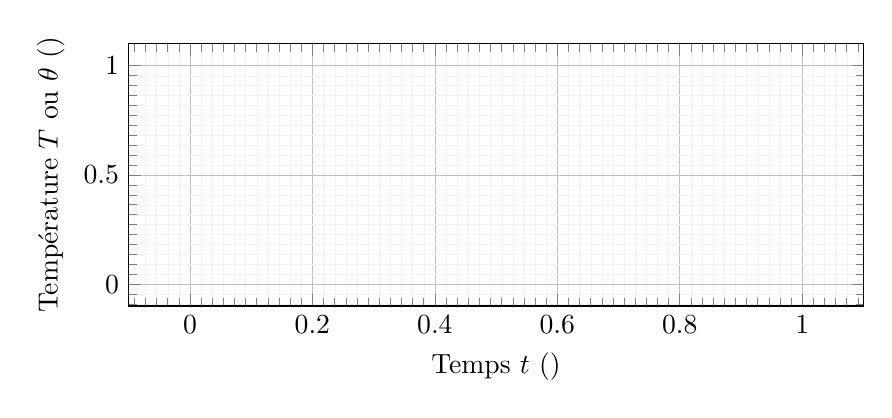
\begin{tikzpicture}
    \def\width{.9*\textwidth};
    \def\height{.45*\width};
    \def\spx{.25cm};
    \def\spy{1.25cm};
    \def\legx{.5cm};
    \def\legy{\legx};
    \def\prop{.45};

    
    \begin{axis}[name=TenuePress,width={\width},height={\height},
    grid=both, minor tick num=10, 
    grid style={line width=.1pt, draw=gray!10},
    major grid style={line width=.2pt,draw=gray!50},
    xlabel={Temps $t$ (\unit{\second})},
    ylabel={Température $T$ ou $\theta$ (\unit{\kelvin})},
%    xmin=0,xmax=75,ymin=0,ymax=.5/1000,
%    xtick={0,25,50,75,100}, ytick={0,1e-4,...,10e-4},
    scaled y ticks = false,
    scaled x ticks = false,
    domain=0:100,
    legend cell align={left},
    legend style = {at={($(1,1)+(-2mm,-2mm)$)},anchor = north east,rounded corners}
    ]
    
    \draw (axis cs:.5,.5) node [rotate=30, text=red] {AJOUTER DONNEES};
%    \addplot[Plasma1, ultra thick] coordinates {(1,1),}

    \end{axis}
\end{tikzpicture}
	\caption{\'Evolution temporelle des températures de part et d'autre de l'échangeur ambiant. \echaf{compléter légende} \echaf{pour l'instant pas trouvé de données qui sont en accord clair avec ça, on laisse tomber ?}}
	\label{fig:TemperatureAHX_InOut}
\end{figure}

\subparagraph{\'Echangeur froid}
L'échangeur froid sert un tout autre but. La caractérisation des performances du réfrigérateur, comme la capacité de refroidissement et le coefficient de performances, repose sur la mesure de la puissance à fournir pour atteindre une certaine température et à s'y stabiliser. Cet échangeur agit donc comme une charge thermique \echaf{fictive} qui fournit cette puissance thermique.

Après un dimensionnement réalisé en suivant la même méthode que pour l'échangeur ambiant, il est fabriqué en aluminium par impression 3D. En revanche, il ne contient pas de fluide qui s'écoule à l'intérieur. À la place, six cartouches chauffantes (Omega, HDC19107) de diamètre \qty{3.2}{\milli\meter} sont placées dans des canaux centraux selon la configuration de la figure~\ref{fig:CHXschema} et dont le diamètre est de \qty{3.6}{\milli\meter} afin de permettre l'application de pâte thermique et améliorer le transfert de chaleur. Ces cartouches sont connectées en parallèle, ce qui donne une résistance électrique de \qty{22.4}{\ohm} aux bornes de l'échangeur et une puissance électrique maximale admise de \qty{600}{\watt}. Autour de ces canaux se trouve \echaf{X} ailettes de dimensions \echaf{toto}, pour une porosité de \qty{40}{\percent}.

La puissance thermique $\dot Q_f$ est apportée par effet Joule au côté froid du noyau selon la relation

\begin{equation}
	\dot Q_f = \frac{E^2}{R},
	\label{eq:Qf_Definition}
\end{equation}
où $E$ est la tension appliquée aux cartouches par un transformateur.



\subsection{Instrumentation}
L'instrumentation utilisée est basée sur celle conçue au début du projet \cite{ramadan_design_2021}, tout en modifiant quelques éléments.

%\bigskip

\subsubsection{Banc d'essais}
La figure~\ref{fig:BancEssaisComplet} présente le banc d'essais complet. Il est possible d'y voir le réfrigérateur et les câbles de connexion des capteurs sur la baie National Instruments \echaf{modèle}, ainsi que l'armoire contenant les bouteilles des gaz nécessaires au mélange utilisé comme fluide de travail, et enfin l'ordinateur pour réaliser les acquisitions.\smallskip

Cette figure permet également d'introduire le repère $(O;\mathbf e_{x,0},\mathbf e_{y,0},\mathbf e_{z,0})$ qui sert de référence pour les orientations décrites dans la figure~\ref{fig:OrientationCore}.

\begin{figure}[!ht]
	\centering
%	\external{•}
%%	\externalremake
%	\input{../fig/•}
%	\tikz{\draw(0,0) node{\includegraphics[width=.95\textwidth]{../fig/•}};}
\includegraphics[width=.7\textwidth]{example-image}
	\caption{Photographie du banc d'essais complet.}
	\label{fig:BancEssaisComplet}
\end{figure}


\subsubsection{Chaîne d'excitation}
La chaîne d'excitation est présentée. Elle n'est pas modifiée durant cette thèse, et se compose d'un générateur de fonction à deux canaux (TekTronix, AFG3022). Chaque canal est ensuite connecté à un amplificateur pour chaque source acoustique. La source principale (RIX Industries, 1S241M) est alimentée par un amplificateur QSC PLD4.5, et la source secondaire (Peerless, GBS135F) par un amplificateur Yamaha P3500S.\medskip


\subsubsection{Chaîne d'acquisition}
La chaîne d'acquisition se compose de plus de trente capteurs. Tous ne sont pas utilisés, mais peuvent servir de contrôle durant une expérience, pour s'assurer du bon déroulement de celle-ci. Les différentes quantités acquises sont détaillé dans cette partie, car quelques modifications ont été apportées au dispositif de mesure mis en place dans le projet \textsc{Tacot} avant le démarrage de cette thèse.

\paragraph{Alimentation électrique des sources} L'alimentation électrique de la source acoustique principale est mesurée au moyen d'une sonde différentielle pour la tension \echaf{et le courant ?}. Pour la source acoustique secondaire, un multimètre  et une pince de courant \echaf{modèle} se chargent de mesurer sa consommation électrique. En parallèle, les tensions aux bornes des deux sources sont affichées sur un oscilloscope pour s'assurer de leur déphasage.

\paragraph{Température} Dix-neuf thermocouples Type K de \qty{.5}{\milli\meter} de diamètre sont placés de la manière suivante : quinze thermocouples mesurent la température en différentes positions du noyau, un devant la source acoustique principale, deux derrière celle-ci, et un derrière la source acoustique secondaire. Cependant, la carte d'acquisition utilisée (National Instruments, NI9213) ne comporte que seize entrées, il faut donc sélectionner les trois thermocouples dont les signaux sont mis de côté, suivant les informations recherchées dans une expérimentation donnée. Dans tous les résultats de mesures discutés dans la suite, les thermocouples du noyau et de devant la source acoustique principale sont connectés. Le placement de ces thermocouples d'intérêt est représenté sur la figure~\ref{fig:TCdansNoyau} par les symboles `\textcolor{cyan}{\textbullet}'.

\begin{figure}[!ht]
    \centering
    \external{fig_TCdansNoyau}
    %\externalremake
    \begin{tikzpicture}[scale=.2]
	\def\rCHX{14cm};
	\def\lCHX{.7cm};
	\def\rREG{14.8cm};
	\def\lREG{3.9cm};
	\def\rAHX{11cm};
	\def\lAHX{2.3cm};
	
	
	\fill[pattern=horizontal lines,pattern color=MatlabOrange,draw=black] (0,-\rAHX) rectangle ++(\lAHX,2*\rAHX);
	\draw[MatlabOrange] (0,-\rAHX) node(AHX)[below left]{\'Echangeur ambiant};
	\foreach \r in {-.9,0,.9}{
		\draw[cyan] (-.15*\lREG,\r*\rAHX) node{\textbullet};
	}
	\filldraw[draw=black,fill=gray!50!white] (0,\rAHX) rectangle (\lAHX,\rREG);		% côtés où l'eau circule
	\filldraw[draw=black,fill=gray!50!white] (0,-\rAHX) rectangle (\lAHX,-\rREG);	%
	
	\draw[MatlabOrange,->] (AHX.north) to[out=90,in=180] (-.1*\lCHX,-.5*\rAHX);
	
	\begin{scope}[xshift=\lAHX] % Reg
		\fill[pattern=crosshatch,pattern color=gray,draw=black] (0,-\rREG) rectangle ++(\lREG,2*\rREG);
		\draw[black] (\lREG/2,\rREG) node[above]{Régénérateur};		
		\foreach \x in {.15,.5,.85}{
			\foreach \r in {-.9,0,.9}{
				\draw[cyan] (\x*\lREG,\r*\rREG) node{\textbullet};
		}}
	\end{scope}
	
	\begin{scope}[xshift=\lAHX+\lREG] % CHX
		\fill[pattern=horizontal lines,pattern color=MatlabBlue,draw=black] (0,-\rCHX) rectangle ++(\lCHX,2*\rCHX);
		\draw[MatlabBlue] (\lCHX,-\rCHX) node(CHX)[below right]{\'Echangeur froid};
		\foreach \r in {-.9,0,.9}{
		\draw[cyan] (\lCHX+.15*\lREG,\r*\rCHX) node{\textbullet};
	}
	\filldraw[draw=black,fill=gray!50!white] (0,\rREG) rectangle (\lCHX,\rCHX);		% côtés où l'eau circule
	\filldraw[draw=black,fill=gray!50!white] (0,-\rREG) rectangle (\lCHX,-\rCHX);	%
	
	\draw[MatlabBlue,->] (CHX.north) to[out=90,in=0] (1.1*\lCHX,-.5*\rCHX);
	\end{scope}
	
	\draw[green!50!black] (0,0) node[left]{\begin{tabular}{rl}Source & \\ acoustique & $\leftarrow$ \\ secondaire &\end{tabular}};
	\draw[green!50!black] ({\lCHX+\lREG+\lAHX},0) node[right]{\begin{tabular}{rl}	
	 & Source \\ $\rightarrow$ \textcolor{cyan}{\textbullet} & acoustique \\ & principale\end{tabular}};
	
\end{tikzpicture}
    \caption{Emplacement des thermocouples choisis pour l'étude thermique dans et autour du noyau thermoacoustique. Zoom sur les encadrés violet et jaune de la figure~\ref{fig:SchemaGeneralTACOT}.}
    \label{fig:TCdansNoyau}
\end{figure}

\paragraph{Pression dynamique} Quatre sondes piézoélectriques (PCB Piezotronics, 113B28) captent les oscillations de pression dans la pompe à chaleur. Deux sont placées à l'arrière de chacune des sources acoustiques, et les deux autres dans le canal de rétroaction de la cavité thermoacoustique, l'un à côté de l'autre. Les capteurs sont ensuite connectés à une carte d'acquisition (National Instruments, NI9234). Cet arrangement est le même depuis la conception de la machine.
%Toutefois, la longueur d'onde dans le mélange de gaz vaut $\lambda=\qty{11.7}{\meter}$ à la fréquence de fonctionnement $f=\qty{47}{\hertz}$ et est suffisamment grande pour garantir une amplitude de pression constante dans toute la machine.

\paragraph{Pression statique} Deux capteurs (Endress, Cerabar PMP21) sont connectés sur les deux tuyaux d'alimentation en gaz de la pompe  à chaleur d'un côté, et sur une carte d'acquisition (National Instruments, NI9234) de l'autre. Les arrivées de gaz se trouvent de part et d'autre de la source acoustique principale et ont pour but d'éviter une surpression sur sa face avant ou arrière et son endommagement. Ici encore, les capteurs sont les mêmes qu'au démarrage de cette thèse.

\paragraph{Puissance extraite par l'échangeur ambiant} Le fonctionnement de cet échangeur est détaillé dans l'annexe~\ref{chap:AHX}. Pour déterminer la quantité de chaleur extraite du côté ambiant du noyau, la différence de température entre l'entrée d'eau de l'échangeur et sa sortie d'eau est mesurée grâce à deux sondes de platine PT100 connectées sur une carte d'acquisition (National Instruments, NI9217). Ici, ce n'est pas l'installation matérielle qui est modifiée mais l'utilisation qui en est faite, pour améliorer la fiabilité de la mesure du flux de chaleur extrait par l'échangeur.

\paragraph{Déplacement des sources} Le piston de chaque source acoustique est équipé d'un accéléromètre. Pour la source acoustique principale, l'accéléromètre (MMF, KS91C), déjà en place au début de cette thèse, est collé sur la face arrière. Pour la source secondaire, le capteur (PCB Piezotronics, 352C23) est collé sur la face avant, après une installation peu conventionnelle détaillée en annexe~\ref{chap:InstrumHP}. Ces capteurs sont choisis de sorte à ne pas trop varier la masse de l'équipage mobile, en particulier pour la source secondaire où la masse du piston et celle de l'ensemble accéléromètre et câble sont du même ordre de grandeur.

\paragraph{Traversées étanches} Toutes les connexions entre l'intérieur de la machine sous haute pression statique et l'extérieur se font via des traversées étanches. Pour les capteurs, il s'agit de HF2-8CU+16K de Spectite, dimensionnées pour \qty{550}{\bar}. Pour les sources acoustique, des traversées du frabricant Solid Sealing Technology sont retenue, avec pour la source acoustique principale le modèle FA17613, et pour la source acoustique secondaire le modèle FA36735. \echaf{materiaux pour le joint ?}

%Les signaux de tensions aux bornes des sources acoustiques sont acquis par une carte d'acquisition (National Instruments, (\echaf{modèle}), après connexion à une sonde de tension (\echaf{modèle}). Deux accéléromètres (\echaf{modèle}) sont collés sur les sources pour mesurer leur déplacement. Pour connaître la pression acoustique dans la cavité thermoacoustique, quatre sondes (\echaf{modèle}) sont placées respectivement à l'arrière de la source principale, à l'arrière de la source secondaire 


%\begin{figure}[!ht]
%    \centering
%    \external{fig_ChaineAcqui}
%    %\externalremake
%    \begin{tikzpicture}
	\draw (0,0) --++(1,0);
\end{tikzpicture}
%    \caption{Carte de la chaine d'acquisition et d'alimentation du réfrigérateur TACOT}
%    \label{fig:ChaineAcqui}
%\end{figure}

%\begin{itemize}
%    \item GBF
%    \item Amplis
%    \begin{itemize}
%        \item QSC
%        \item Yamaha
%    \end{itemize}
%    \item Sondes de tension
%    \item Cartes NI
%    \begin{itemize}
%        \item Pression statique
%        \item Pression dynamique
%        \item Thermocouples
%        \item PT100
%        \item Accéléromètres
%    \end{itemize}
%    \item LabVIEW d'acquisition
%\end{itemize}

%Pour étudier la distribution de température le long de l'axe du noyau, ainsi que dans les dimensions transverses, Seize thermocouples sont placés sur un plan et représentés par les symboles~`\textcolor{cyan}{\textbullet}' sur la figure~\ref{fig:TCdansNoyau}. Neuf sont placés au c\oe{}ur du noyau, dans le régénérateur. Trois sont fixés à l'extérieur du noyau, hors de l'échangeur ambiant, et trois autres sur l'extérieur de l'échangeur froid. Enfin, un dernier thermocouple est positionné au voisinage de la source acoustique principale, en vis-à-vis de l'échangeur froid.



%\subsection{Emplacement des capteurs}
%
%\begin{figure}[!ht]
%    \centering
%    \external{fig_ThermocouplesDefinition}
%    %\externalremake
%    \begin{tikzpicture}
    \def\LX{1};
    \def\LY{2};
    \def\CoreX{1.5};
    \def\CoreY{.9*\LY};
    
    \draw[line width=.5mm] (-2.5*\LX,0) to[out=90,in=-180] (-\LX,\LY) -- ++(2*\LX,0) -- ++(.5*\LX,-2*\LY/3) -- ++(.2*\LX,0) -- ++(0,2*\LY/3);
\draw[line width=.5mm] (\LX,\LY) -- ++(\LX,0) to[out=0,in=90] (3.5*\LX,0);

\draw[line width=.5mm] (-\LX,\CoreY) -- ++(\CoreX,0);
\draw[fill=PythonBlue] (-.9*\LX,0) -- ++(0,\CoreY) to[out=-80,in=90] (-.7*\LX,0);
\draw ({-\LX+.4*\CoreX},0) -- ++(0,\CoreY);
\draw ({-\LX+.9*\CoreX},0) -- ++(0,\CoreY);

\draw[fill=PythonBlue] (1.6*\LX,0) |- ++(.3*\LX,.9*\LY/3) |- ++(\LX,.2*\LY) arc (90:0:.05) -- ++(0,-.5*\LY);
    
    \begin{scope}[xscale=1,yscale=-1]
        \draw[line width=.5mm] (-2.5*\LX,0) to[out=90,in=-180] (-\LX,\LY) -- ++(2*\LX,0) -- ++(.5*\LX,-2*\LY/3) -- ++(.2*\LX,0) -- ++(0,2*\LY/3);
\draw[line width=.5mm] (\LX,\LY) -- ++(\LX,0) to[out=0,in=90] (3.5*\LX,0);

\draw[line width=.5mm] (-\LX,\CoreY) -- ++(\CoreX,0);
\draw[fill=PythonBlue] (-.9*\LX,0) -- ++(0,\CoreY) to[out=-80,in=90] (-.7*\LX,0);
\draw ({-\LX+.4*\CoreX},0) -- ++(0,\CoreY);
\draw ({-\LX+.9*\CoreX},0) -- ++(0,\CoreY);

\draw[fill=PythonBlue] (1.6*\LX,0) |- ++(.3*\LX,.9*\LY/3) |- ++(\LX,.2*\LY) arc (90:0:.05) -- ++(0,-.5*\LY);
    \end{scope}
    
    
    \draw[dashed,rounded corners,PythonRed] (.55,.95*\LY) rectangle ++(-.75*\CoreX,-1.9*\LY) node[midway]{\rotatebox{90}{Noyau TA}};
    
    \begin{scope}[xshift=5cm,xscale=2.5,yscale=2]
        \draw (0,0) |- ++(2,1.5) -- ++(0,-1.5);
        \draw (.5,0) -- ++(0,1.5);
        \draw (1.5,0) -- ++(0,1.5);
        \draw[line width=1mm] (-.2,1.5) -- ++(2.4,0);
    
        \begin{scope}[xscale=1,yscale=-1]
            \draw (0,0) |- ++(2,1.5) -- ++(0,-1.5);
            \draw (.5,0) -- ++(0,1.5);
            \draw (1.5,0) -- ++(0,1.5);
            \draw[line width=1mm] (-.2,1.5) -- ++(2.4,0);
        \end{scope}
        % \foreach \x [evaluate=\x] in {0,...,4}{
        %     \foreach \y [evaluate=\y] in {1,...,3}{
        %     \draw (\x,\y) node[]{$t$};}}
    \end{scope}
    
    %\draw[line width=1mm] (5*\LX,.5*\LY) -- ++(6*\LX,0);
    %\draw[line width=1mm] (5*\LX,-.5*\LY) -- ++(6*\LX,0);
    %
    %\draw (-2.5*\LX,\LY) node[above]{\bf (a)};
    %\draw (5*\LX,\LY) node[above]{\bf (b)};
    
\end{tikzpicture}
%    \caption{Emplacements des thermocouples dans le noyau thermoacoustique}
%    \label{fig:ThermocouplesDefinition}
%\end{figure}

\section{Protocole expérimental}\label{chap:ProtocolExpe}
Pour l'étude de l'influence de la gravité sur la distribution de température dans son noyau et ses performances, le réfrigérateur doit pouvoir être orienté dans toutes les orientations utiles. Pour ce faire, il est suspendu par des palans grâce aux fixations situées à ses extrémité  et au milieu dans le sens de sa longueur. La figure~\ref{fig:TACOTSuspendu_Frigo} présente le réfrigérateur accroché à ses extrémités, et la figure~\ref{fig:TACOTSuspendu_Palans} les trois palans pour le soutenir. Les deux palans de couleur grise, initialement présents pour régler l'inclinaison de la pompe à chaleur par rapport à l'axe horizontal, et le troisième de couleur bleue pour ajouter une direction de rotation autour de l'axe de symétrie. Celui-ci permet en outre de plus aisément passer d'une orientation à l'autre. 

\begin{figure}[!ht]
    \centering
	\begin{subfigure}{.45\textwidth}
		\centering
		\external{fig_SystemeAccroche_Machine}
		\tikz{\draw(0,0) node{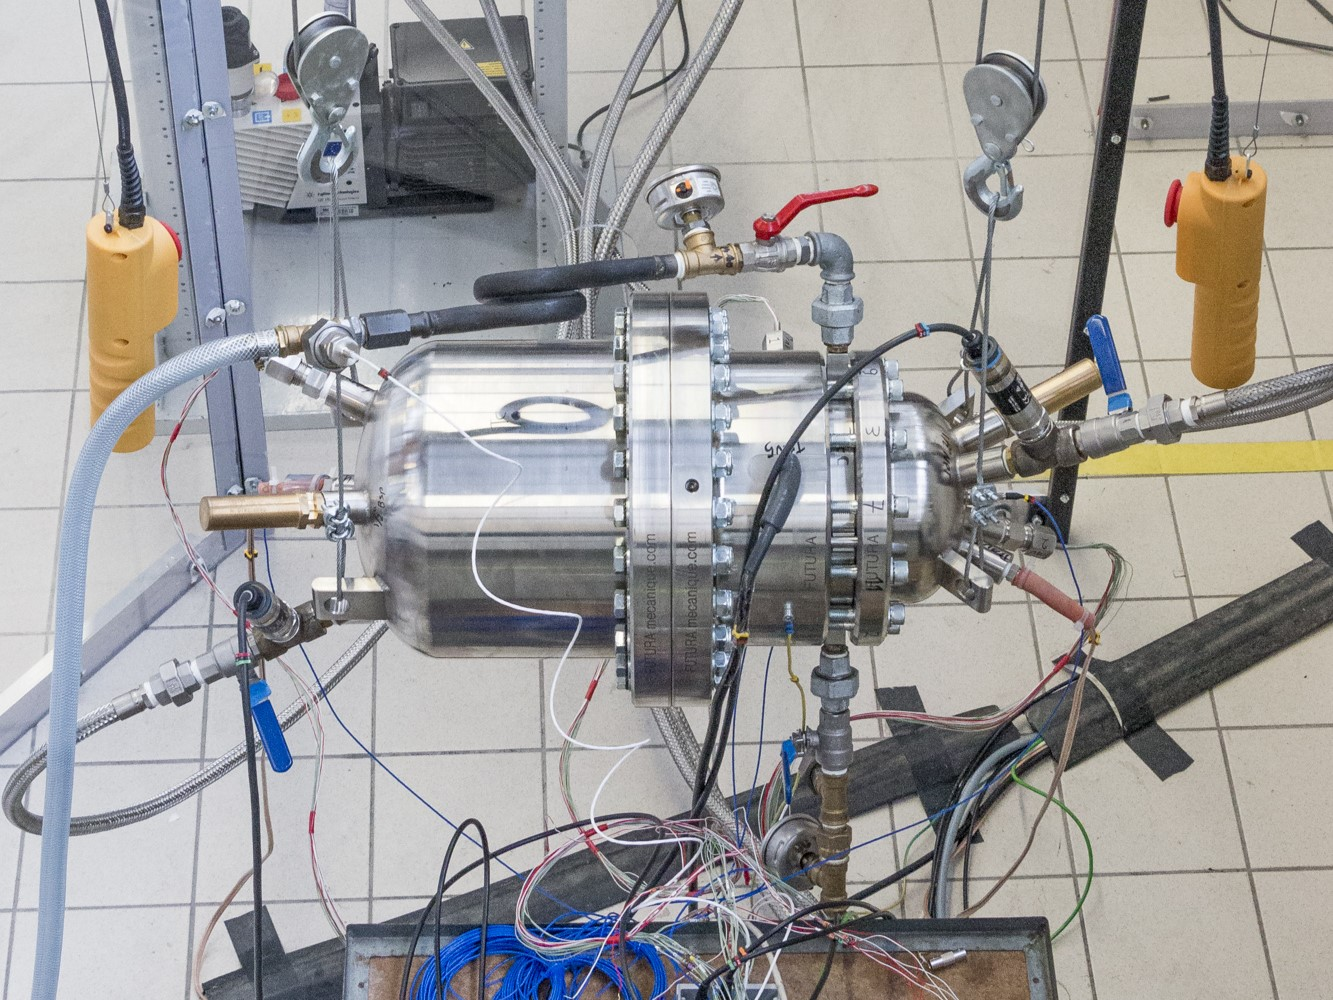
\includegraphics[width=.9\textwidth]{../fig/fig_SystemeAccroche/Machine_horizBetter_cropped.jpg}};}
		\caption{}
		\label{fig:TACOTSuspendu_Frigo}
	\end{subfigure}		%
	\begin{subfigure}{.45\textwidth}
		\centering
		\external{fig_SystemeAccroche_Palan}
		\tikz{\draw(0,0) node{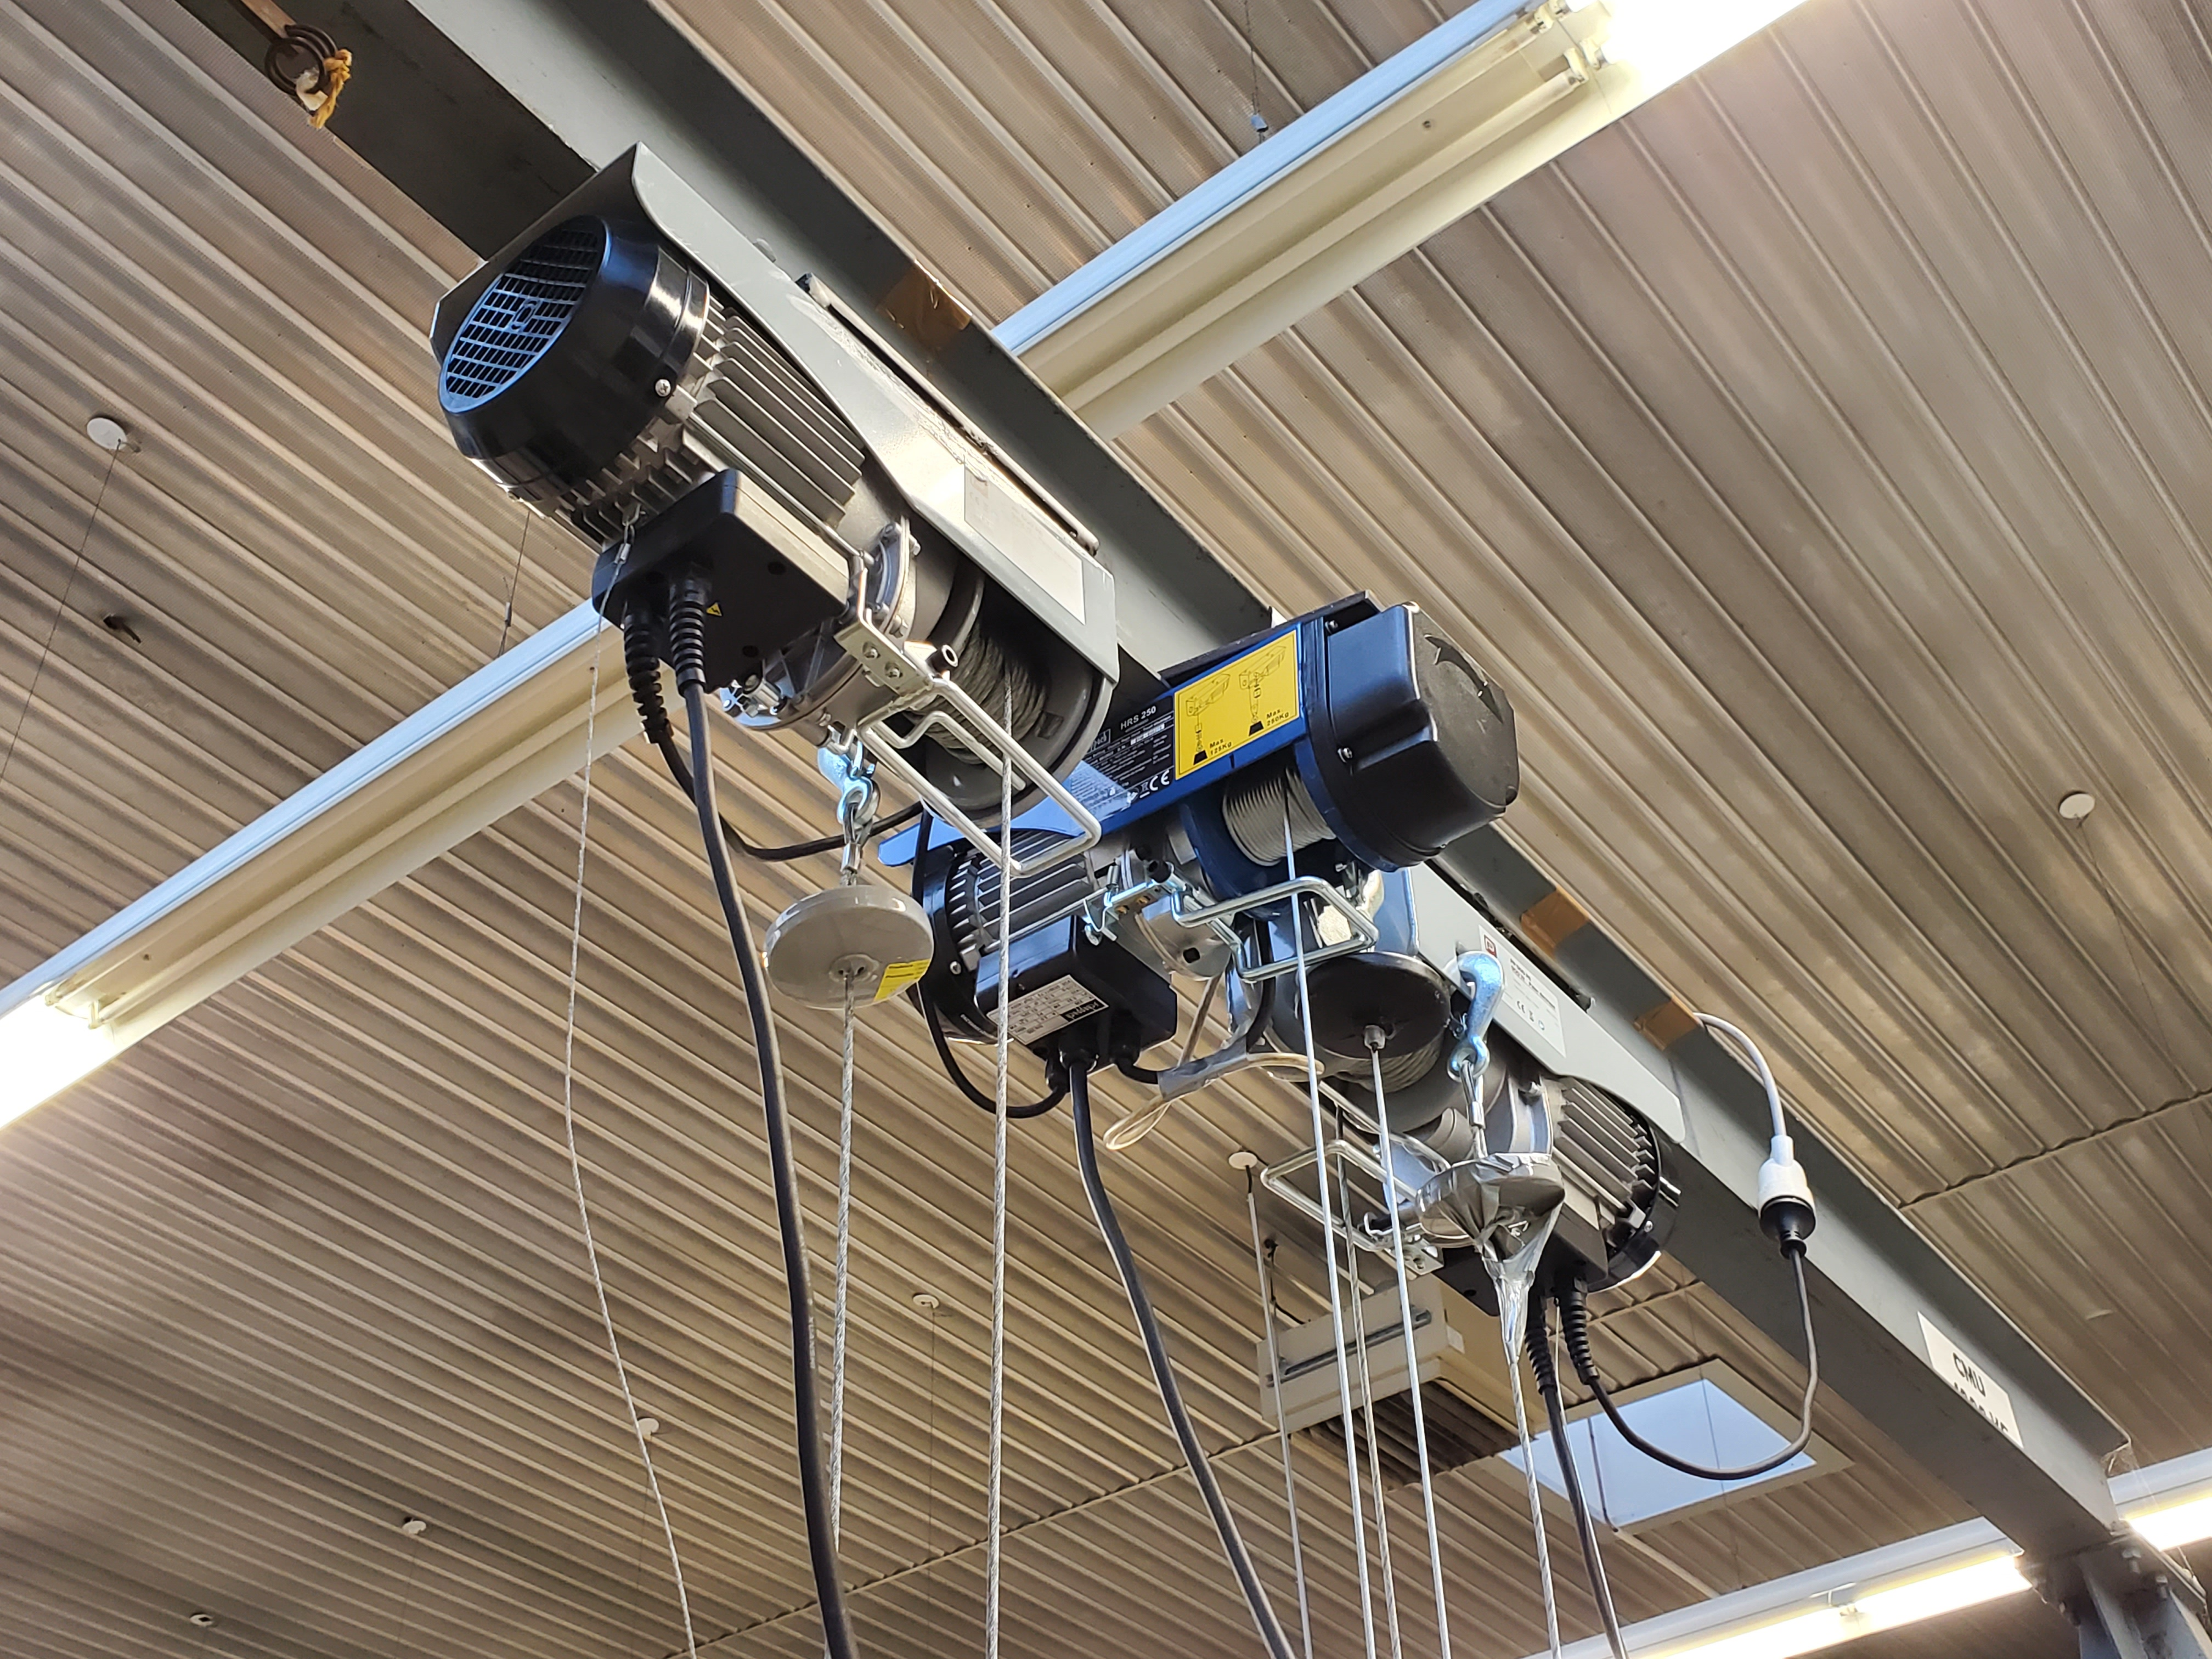
\includegraphics[width=.9\textwidth]{../fig/fig_SystemeAccroche/Palans.jpg}};}
		\caption{}
		\label{fig:TACOTSuspendu_Palans}
	\end{subfigure}	    
    \caption{Photographies \subref{fig:TACOTSuspendu_Frigo} du refrigérateur accroché et \subref{fig:TACOTSuspendu_Palans} des palans formant le système de suspension.}
    \label{fig:TACOTSuspendu}
\end{figure}

Une méthode d'acquisition est également mise en place pour garantir des résultats utilisable pour évaluer les effets de la convection naturelle sur le comportement du réfrigérateur. Ce protocole est développé après une grande quantité d'expériences non-concluantes, et est décrit ci-après.

\subsection{Définition des orientations}
Quelques questions sont formulées, auxquelles il faut répondre en choisissant judicieusement des configurations expérimentales adaptées. 

L'étude expérimentale menées ici doit permettre de comprendre comment se manifeste une cellule de convection naturelle, et si l'hypothèse d'axisymétrie posée lors de la conception de la machine reste valide en cas de présence de convection naturelle. Il faut ensuite évaluer si une configuration est plus favorable à la mise en place d'une ou plusieurs cellules de convection naturelle dans le \textsc{Tacot}, et si les performances sont affectées par elles. L'existence de volumes de gaz poreux ou non interroge également sur la possibilité d'un écoulement de fluide dans le régénérateur, et sur son impact éventuel.\medskip 

Les orientations retenues pour le travail présenté dans ce manuscrit sont judicieusement choisies pour leur caractère académique -- avec un gradient de température soit vertical, soit horizontal --, et sont présentées sur la figure~\ref{fig:OrientationCore}. La gravité y est toujours dirigée vers le bas de la page, et les numéros d'identification des thermocouples utilisés et dont l'emplacement est noté sur la figure~\ref{fig:TCdansNoyau} y est détaillé.\medskip

\begin{figure}[!htp]
	\centering		
	\begin{subfigure}[c]{.4\textwidth}
		\centering
		\external{fig_OrientationCore_H1}
%    	\externalremake
		\begin{tikzpicture}[scale=2/3]

%    \def\lenreg{2};
%    \def\diam{3};
    \def\spy{2};
    \def\xdist{8cm};
    \def\ydist{-7cm};
%    \def\persp{20};
%    
%    \def\LX{1};
%    \def\LY{2};
%    \def\CoreX{1.5};
%    \def\CoreY{.9*\LY};
%    

	\def\L{2.1};
	\def\R{5};
	\def\HX{.25};
	\def\decalage{\R/2-\L/2};
	
		\draw(6.5,\R/2) node{\includegraphics[width=.8\textwidth]{../fig/fig_OrientationCore/tex/TACOT.png}};
			
		\fill[right color=blue!25,left color=red!25, draw=black] (\decalage,0) rectangle ++(\L,\R);
		\draw[fill=red!25] (\decalage,0) rectangle ++(-\HX,\R);
		\draw[fill=blue!25] (\decalage+\L,0) rectangle ++(\HX,\R);

		\foreach \z [evaluate=\z] in {0,...,4}{
			\foreach \r [evaluate=\r as \num using int(\r+1 + 3*\z)] in {0,...,2}{
				\draw ({\decalage+.5+\L-\z*(1+\L)/4},{-(\R-.4)/2*\r+\R-.2}) node[minimum size=10pt,draw,circle,fill=white,opacity=.7,text opacity=1]{} node(n\z\r){\scriptsize \num};
}}

%		\draw (n01.east) node [right]{0 $\rightarrow$ \begin{tabular}{l}Source\\acoustique\\principale\end{tabular}};
		\draw ($(n01)+(1.5,0)$) node[minimum size=10pt,draw,circle,fill=white,opacity=.7,text opacity=1]{} node(RIX) {\scriptsize 0};% node[anchor=west]{\begin{tabular}{rl}
%		& Source\\
%		$\rightarrow$ & acoustique\\
%		& principale
%		\end{tabular}};
		\draw (n30.north west) node [above, fill=white, fill opacity=.7, text opacity=1]{Ambiant};
		\draw (n10.north east) node [above, fill=white, fill opacity=.7, text opacity=1]{Froid};
\end{tikzpicture}
		\caption{}
		\label{fig:OrientationCore_H1}
	\end{subfigure} 
	\begin{subfigure}[c]{.4\textwidth}
		\centering
		\external{fig_OrientationCore_H2}
%    	\externalremake
		\begin{tikzpicture}[scale=2/3]

%    \def\lenreg{2};
%    \def\diam{3};
    \def\spy{2};
    \def\xdist{8cm};
    \def\ydist{-7cm};
%    \def\persp{20};
%    
%    \def\LX{1};
%    \def\LY{2};
%    \def\CoreX{1.5};
%    \def\CoreY{.9*\LY};
%    

	\def\L{1};
	\def\R{5};
	\def\HX{.25};
	\def\decalage{\R/2-\L/2};
	
%	\draw[opacity=0] (\decalage,0) rectangle ++(-\HX,\R); %%% Pour l'alignement vertical
%\draw{[white](\L/2,0) -- ++(0,\R);
	
	\begin{scope}[yslant=-1]
		\begin{scope}[xslant=.71]%, rotate=90, xscale=1]
		\node at (\decalage-\HX,0) (NewO) {};
%		\draw[->, very thick] (NewO.center) -- ++(0,1.2*\R);
%		\draw[->, very thick] (NewO.center) -- ++(1.2*\R,0);
		
		\fill[shading=axis,right color=MatlabBlue,left color=MatlabOrange, shading angle=22.5, draw=black] (\decalage,0) rectangle ++(\L,\R*1.4);
		\draw[fill=MatlabOrange] (\decalage,0) rectangle ++(-\HX,\R*1.4);
		\draw[fill=MatlabBlue] (\decalage+\L,0) rectangle ++(\HX,\R*1.4);

		\foreach \z [evaluate=\z] in {0,...,4}{
			\foreach \r [evaluate=\r as \num using int(\r+1 + 3*\z)] in {0,...,2}{
				\draw ({\decalage+.5+\L-\z*(1+\L)/4},{-(\R*1.4-.4)/2*\r+\R*1.4-.2}) node[minimum size=10pt,draw,circle,fill=white,opacity=.7,text opacity=1]{} node(n\z\r){\scriptsize \num};
}}

%		\draw (n01.east) node [right]{$\rightarrow$ \begin{tabular}{l}Source\\acoustique\\principale\end{tabular}};
		\draw ($(n01)+(.75,0)$) node[minimum size=10pt,draw,circle,fill=white,opacity=.7,text opacity=1]{} node {\scriptsize 0};% node[anchor=west]{\begin{tabular}{rl}
%		& Src\\
%		$\rightarrow$ & ac\\
%		& princ
%		\end{tabular}};
%		\draw (n30.north west) node [above right, fill=white, fill opacity=0, text opacity=1]{\textcolor{MatlabOrange}{\textbf{Ambiant}}};
%		\draw (n10.north east) node [above right, fill=white, fill opacity=0, text opacity=1]{\textcolor{MatlabBlue}{\textbf{Froid}}};
		
	\end{scope}
	\end{scope}
	\begin{pgfonlayer}{background}
		\draw[->, very thick] (NewO.center) -- ++(22.5:1.2*\R) node [above] {$\mathbf e_{y,0}$};
		\draw[->, very thick] (NewO.center) -- ++(90:1.2*\R) node [left] {$\mathbf e_{z,0}$};
		\draw[->, very thick] (NewO.center) -- ++(-45:1.2*\R) node [right] {$\mathbf e_{x,0}$};
  	\end{pgfonlayer}
\end{tikzpicture}
		\caption{}
		\label{fig:OrientationCore_H2}
	\end{subfigure} 

	\vspace{1cm}
	
	\begin{subfigure}[c]{.4\textwidth}
		\centering
		\external{fig_OrientationCore_V1}
%    	\externalremake
		%\fill[top color=red!25, bottom color=blue!25, draw=black] (0,0) rectangle ++(\R,\L);
%\draw[fill=blue!25] (0,0) rectangle ++(\R,-\HX);
%\draw[fill=red!25] (0,\L) rectangle ++(\R,\HX);
%
%\foreach \z [evaluate=\z] in {0,...,4}{
%	\foreach \r [evaluate=\r as \num using int(\r+1 + 3*\z)] in {0,...,2}{
%		\draw ({-(\R-.4)/2*\r+\R-.2},{\z*(1+\L)/4-.5}) node(n\z\r){\num};
%}}
%
%\draw (n40.south east) node [right]{AHX};
%\draw (n00.north east) node[right]{CHX};
%\draw (n01.south) node [below]{\shortstack{ $\downarrow$ \\Source acoustique principale}};
%
%\draw (0,\L+2*\HX+\spy) node [anchor=west]{\textbf{(c)} \texttt{V1}};

\begin{tikzpicture}[scale=2/3]

%    \def\lenreg{2};
%    \def\diam{3};
    \def\spy{2};
    \def\xdist{8cm};
    \def\ydist{-7cm};
%    \def\persp{20};
%    
%    \def\LX{1};
%    \def\LY{2};
%    \def\CoreX{1.5};
%    \def\CoreY{.9*\LY};
%    

	\def\L{2};
	\def\R{5};
	\def\HX{.35};
	\def\decalage{\R/2-\L/2};
	
	\begin{scope}[yslant=tan(22.5)]	
		
		\node at (0,-\HX) (NewO) {};
	
		\fill[shading=axis,right color=MatlabBlue,left color=MatlabOrange, shading angle=22.5, draw=black] (0,0) rectangle ++(\R,\L);
		\draw[fill=MatlabBlue] (0,0) rectangle ++(\R,-\HX);
		\draw[fill=MatlabOrange] (0,\L) rectangle ++(\R,\HX);

		\foreach \z [evaluate=\z] in {0,...,4}{
			\foreach \r [evaluate=\r as \num using int(\r+1 + 3*\z)] in {0,...,2}{
				\draw ({-(\R-.4)/2*\r+\R-.2},{\z*(1+\L)/4-.5}) node[minimum size=10pt,draw,circle,fill=white,opacity=.7,text opacity=1]{} node(n\z\r){\scriptsize \num};
}}

%		\draw (n40.south east) node [right, fill=white, fill opacity=0, text opacity=1]{\textcolor{MatlabOrange}{\textbf{Ambiant}}};
%		\draw (n00.north east) node[right, fill=white, fill opacity=0, text opacity=1]{\textcolor{MatlabBlue}{\textbf{Froid}}};
		\draw ($(n01.south)+(0,-1.1)$) node[minimum size=10pt,draw,circle,fill=white,opacity=.7,text opacity=1]{} node (RIX){\scriptsize 0};% node[anchor=north]{\begin{tabular}{c}
%		$\downarrow$\\
%		Source acoustique principale
%		\end{tabular}};

	\end{scope}
	\begin{pgfonlayer}{background}
		\draw[->, very thick] (NewO.center) -- ++(22.5:1.2*\R) node [above] {$\mathbf e_{y,0}$};
		\draw[->, very thick] (NewO.center) -- ++(90:1.2*\R) node [left] {$\mathbf e_{z,0}$};
		\draw[->, very thick] (NewO.center) -- ++(-45:1.2*\R) node [right] {$\mathbf e_{x,0}$};
  	\end{pgfonlayer}		
\end{tikzpicture}
		\caption{}
		\label{fig:OrientationCore_V1}
	\end{subfigure} 
	\begin{subfigure}[c]{.4\textwidth}
		\centering
		\external{fig_OrientationCore_V2}
%    	\externalremake
		%\fill[top color=blue!25, bottom color=red!25, draw=black] (0,0) rectangle ++(\R,\L);
%\draw[fill=red!25] (0,0) rectangle ++(\R,-\HX);
%\draw[fill=blue!25] (0,\L) rectangle ++(\R,\HX);
%
%\foreach \z [evaluate=\z] in {0,...,4}{
%	\foreach \r [evaluate=\r as \num using int(\r+1 + 3*\z)] in {0,...,2}{
%		\draw ({(\R-.4)/2*\r+.2},{-\z*(1+\L)/4+\L+.5}) node(n\z\r){\num};
%}}
%
%\draw (n01.north) node [above]{\shortstack{Source acoustique principale\\ $\uparrow$}};
%\draw (n42.north east) node [right]{AHX};
%\draw (n02.south east) node [right]{CHX};
%
%\draw (0,\L+2*\HX+\spy) node [anchor=west]{\textbf{(d)} \texttt{V2}};

\begin{tikzpicture}[scale=2/3]

%    \def\lenreg{2};
%    \def\diam{3};
    \def\spy{2};
    \def\xdist{8cm};
    \def\ydist{-7cm};
%    \def\persp{20};
%    
%    \def\LX{1};
%    \def\LY{2};
%    \def\CoreX{1.5};
%    \def\CoreY{.9*\LY};
%    

	\def\L{2.1};
	\def\R{5};
	\def\HX{.25};
	\def\decalage{\R/2-\L/2};

		\fill[top color=MatlabBlue, bottom color=MatlabOrange, draw=black] (0,0) rectangle ++(\R,\L);
		\draw[fill=MatlabOrange] (0,0) rectangle ++(\R,-\HX);
		\draw[fill=MatlabBlue] (0,\L) rectangle ++(\R,\HX);

		\foreach \z [evaluate=\z] in {0,...,4}{
			\foreach \r [evaluate=\r as \num using int(\r+1 + 3*\z)] in {0,...,2}{
				\draw ({(\R-.4)/2*\r+.2},{-\z*(1+\L)/4+\L+.5}) node[minimum size=10pt,draw,circle,fill=white,opacity=.7,text opacity=1]{} node(n\z\r){\scriptsize \num};
}}

		\draw ($(n01.north)+(0,1.1)$) node[minimum size=10pt,draw,circle,fill=white,opacity=.7,text opacity=1]{} node(RIX){\scriptsize 0};% node[anchor=south]{\begin{tabular}{c}
%		Source acoustique principale\\
%		$\uparrow$
%		\end{tabular}};
		\draw (n42.north east) node [right, fill=white, fill opacity=.7, text opacity=1]{\textcolor{MatlabOrange}{\textbf{Ambiant}}};
		\draw (n02.south east) node [right, fill=white, fill opacity=.7, text opacity=1]{\textcolor{MatlabBlue}{\textbf{Froid}}};
%		\draw (n41.south) node [below]{\textcolor{white}{\shortstack{Source acoustique principale\\ $\uparrow$}}};
		
\end{tikzpicture}
		\caption{}
		\label{fig:OrientationCore_V2}
	\end{subfigure}  	
 	\caption{Orientations choisies pour les expériences avec le réfrigérateur thermoacoustique, avec les positions des thermocouples et leurs numéro. Pour chaque cas, la gravité est orientée vers le bas de la page, soit $\mathbf g=-g\mathbf e_{z,0}$ suivant le repère défini sur la figure~\ref{fig:BancEssaisComplet}. Les orientations sont \subref{fig:OrientationCore_H1}  `\texttt{H1}', \subref{fig:OrientationCore_H2} `\texttt{H2}',  \subref{fig:OrientationCore_V1} `\texttt{V1}', et  \subref{fig:OrientationCore_V2} `\texttt{V2}'.}%\textcolor{red}{CHX et AHX OK ou éch. froid et éch. chaud ? + $\psi_i$ dans la caption ou la figure ?}}
    \label{fig:OrientationCore} %
\end{figure}


La première orientation, nommée `\texttt{H1}' et représentée sur la figure~\ref{fig:OrientationCore_H1}, est la même que dans l'article dédié à la conception du réfrigérateur \cite{ramadan_design_2021}. Dans cette configuration, le \textsc{Tacot} est placé à l'horizontale comme sur la figure~\ref{fig:TACOTSuspendu_Frigo}, et les thermocouples sont placés sur un plan vertical coplanaire à la gravité. Cette orientation est celle avec laquelle tous les résultats ont été obtenus avant le démarrage de la thèse et fait donc office de référence des orientations.\smallskip

Ensuite, la deuxième orientation est représentée sur la figure~\ref{fig:OrientationCore_H2}. Dans ce cas, référencé en tant que `\texttt{H2}', le réfrigérateur est toujours à l'horizontale, mais pivoté autour de son axe pour placer les thermocouples sur un plan horizontal auquel la gravité est orthogonale.\smallskip

L'orientation `\texttt{V1}' est affichée sur la figure~\ref{fig:OrientationCore_V1}. Cette configuration est radicalement différentes des deux précédentes : l'axe de symétrie du réfrigérateur est vertical, avec l'échangeur froid sous l'échangeur ambiant.\smallskip

Enfin, l'orientation `\texttt{V2}' affichée sur la figure~\ref{fig:OrientationCore_V2} est l'orientation inverse de la précédente. L'axe de symétrie du réfrigérateur est encore vertical, mais l'échangeur froid est cette fois au-dessus de l'échangeur ambiant.\medskip

Ces orientations correspondent à des configurations asymptotiques de convection naturelle, classiques dans la littérature concernée : les orientations horizontales `\texttt{H1}' et `\texttt{H2}' s'approchent du cas d'une cavité différentiellement chauffée, où le gradient de température est horizontal, tandis que les orientations verticales `\texttt{V1}' et `\texttt{V2}' constituent une configuration de Rayleigh-Bénard. Dans le cadre de cette thèse, les orientations intermédiaires ne sont pas testées. Cependant, une étude numérique du réfrigérateur modèle l'impact de la convection naturelle pour d'autres orientation, notamment dans le cas où le noyau est incliné de \ang{45} \cite{baltean_gravity_2025}.\bigskip

Il est important de noter que dans le cas de ce système qui est axisymérique, les orientations horizontales `\texttt{H1}' et `\texttt{H2}' sont dans le principe une même orientation et pour laquelle le double d'information thermique peut \textit{a priori} être extrait.\medskip



%\echaf{rajouter ce que j'ai dit au début : quelle orientation est favorable à la conv nat ? qu'est-ce qu'on s'attend à voir ?}

\subsection{Acquisitions}\label{chap:Acquisitions}
%\echaf{Me faire mousser car je suis "expérimentateur hors pair" ! faire voir le fait qu'il y a peu de résultats mais qu'ils sont le fruit de beaucoup d'essais pour avoir un protocole aux petits oignons et qu'on peut avoir confiance dedans} 
Les acquisitions sont réalisées en plusieurs temps, afin de garantir des résultats exploitables et propres. Le protocole suivant constitue la dernière itération d'une longue série d'acquisitions, dans laquelle chaque campagne comporte quelque chose rendant la mesure inexploitable.

Tout d'abord et pour toutes les expériences,  l'état initial de toutes les grandeurs est acquis sur une minute et sauvegardé sous un label `\texttt{init}' à chaque début de journée de campagne. Cela permet de garder en mémoire toutes les conditions expérimentales initiales dont les valeurs peuvent potentiellement influer sur le comportement du réfrigérateur, comme par exemple la température ambiante ou la pression statique. \smallskip

Ensuite, en prévision de la mesure de flux de chaleur $\dot Q_a$ extrait par l'échangeur ambiant (voir l'annexe~\ref{chap:AHX}), l'eau est préalablement mise en circulation dans cet échangeur après avoir démarré une acquisition des 30 capteurs jusqu'à stabilisation de l'écart de température entre l'entrée et la sortie de la circulation d'eau dans l'échangeur ambiant et la distribution de température dans le noyau. L'acquisition, qui dure entre \qtylist{30;60}{\minute}, est ensuite interrompue et enregistrée avec un label `\texttt{Water}'. Un exemple d'acquisition de ce type est représenté sur la figure~\ref{fig:WaterOnly}, ce qui permet d'apprécier l'ordre de grandeur du temps nécessaire pour réaliser cette étape préliminaire. Il est également notable que la distribution de température  n'est pas encore stabilisée au bout d'\qty{1}{\hour}, tandis que l'écart de température d'eau devient constant au bout de \qty{20}{\minute}. Toutefois, les variations temporelles des températures mesurées dans le noyau sont suffisamment faible pour considérer qu'un état d'équilibre est atteint et que les conditions initiales avant démarrage des sources sont les mêmes d'une expérience à l'autre.\medskip

\begin{figure}[!ht]
    \centering
	\begin{subfigure}{\textwidth}
		\centering
		\external{fig_WaterOnly_TC}
%		\externalremake
		\begin{tikzpicture}
    \def\width{.9*\textwidth};
    \def\height{.25*\textheight};
    \def\legx{.5cm};
    \def\legy{\legx};
    
    \begin{axis}[name=plot,width={\width},height={\height},grid=both,minor tick num=4,
    grid style={line width=.1pt, draw=gray!10},
    major grid style={line width=.2pt,draw=gray!50},
    xlabel={Temps $t$ [\unit{\s}]},
    ylabel={\'Ecart de température $\theta$ [\unit{\kelvin}]},
    xmin=0,xmax=3500,
%	ymin=-5,ymax=50,
    xtick={0,600,...,3000,3500},%ytick={0,9.1120/100000,1.4452/10000,2.5/10000,5/10000,1/1000},
    domain=0:100,
    legend style = {at={(1.01,1.05)},anchor = north east, cells={align=right},rounded corners},legend columns=5,
    ]
    	
    	\addplot[ultra thick,Plasma85] file {{../fig/fig_WaterOnlyExample/data/Water_TC2.txt}};\addlegendentry{TC 2}
    	
    	\addplot[ultra thick,Plasma64] file {{../fig/fig_WaterOnlyExample/data/Water_TC5.txt}};\addlegendentry{TC 5}
    	
    	\addplot[ultra thick,Plasma43] file {{../fig/fig_WaterOnlyExample/data/Water_TC8.txt}};\addlegendentry{TC 8}
    	
    	\addplot[ultra thick,Plasma22] file {{../fig/fig_WaterOnlyExample/data/Water_TC11.txt}};\addlegendentry{TC 11}
    	
    	\addplot[ultra thick,Plasma1] file {{../fig/fig_WaterOnlyExample/data/Water_TC14.txt}};\addlegendentry{TC 14}
    	  
    \end{axis}
%    \draw (plot.center) node[rotate=30]{\color{red}AFFICHER LES DONNEES};
\end{tikzpicture}
		\caption{}
		\label{fig:WaterOnly_TC}
	\end{subfigure}
		
	\vspace{1em}
	
	\begin{subfigure}{\textwidth}
		\centering
		\external{fig_WaterOnly_PT}
%		\externalremake
		\begin{tikzpicture}
    \def\width{.9*\textwidth};
    \def\height{.25*\textheight};
    \def\legx{.5cm};
    \def\legy{\legx};
    
    \begin{axis}[name=plot,width={\width},height={\height},grid=both,minor tick num=4,
    grid style={line width=.1pt, draw=gray!10},
    major grid style={line width=.2pt,draw=gray!50},
    xlabel={Temps $t$ [\unit{\s}]},
    ylabel={\'Ecart de température $\theta$ [\unit{\kelvin}]},
    xmin=0,xmax=3500,
%	ymin=-5,ymax=50,
    xtick={0,600,...,3000,3500},%ytick={0,9.1120/100000,1.4452/10000,2.5/10000,5/10000,1/1000},
    domain=0:100,
    legend style = {at={(1.01,1.05)},anchor = north east, cells={align=right},rounded corners},legend columns=3,
    ]
    	
    	
    	\addplot[ultra thick,black] file {{../fig/fig_WaterOnlyExample/data/Water_PT.txt}};%\addlegendentry{TC 14}
    	
    \end{axis}
%    \draw (plot.center) node[rotate=30]{\color{red}AFFICHER LES DONNEES};
\end{tikzpicture}
		\caption{}
		\label{fig:WaterOnly_PT}
	\end{subfigure}	    
    \caption{Exemple de mesure `\texttt{water}', dans le cas de l'orientation `\texttt{H1}'. \subref{fig:WaterOnly_TC} thermocouples sur le centre du noyau, c'est-à-dire les TC \numlist{2;5;8;11;14}, et \subref{fig:WaterOnly_PT} la différence de température entre la sortie et l'entrée de l'échangeur. Cet exemple est extrait de la campagne `\texttt{heat\_only}' pour l'orientation `\texttt{V1}'.}
    \label{fig:WaterOnly}
\end{figure}

L'étape suivante dépend du type d'expérience menée : les mesures peuvent être sans ou avec acoustique, et ce, pour  différentes amplitudes de pression oscillante. %\echaf{la suite part en intro sur ce qui existe déjà} En revanche, certains des paramètres d'excitation restent constants pour toutes les expériences :  le gaz est également le même dans toutes les expériences. Il est composé de \qty{65}{\percent} d'hélium et de \qty{35}{\percent} d'argon, car dans ces proportions le nombre de Prandtl est minimum \cite{belcher_working_1999} ; ce mélange est ensuite pressurisé à \qty{40}{\bar}. Dans le cas des expériences avec acoustique, le modèle \textsc{DeltaEC} prédit les meilleurs performances à la fréquence $f=\qty{47}{\hertz}$, c'est-à-dire la fréquence de résonance du système. C'est par ailleurs le seul point de fonctionnement où l'impédance électrique est supérieure à la limite basse admise par l'amplificateur, soit \qty{2}{\ohm}. Ensuite, le déphasage inter-source $\varphi_{2-1}$ est également fixé à \ang{-60} pour toutes les expériences, également indiqué comme déphasage optimale par les simulations et que des expériences préliminaires confirment.

\subsubsection{Mesures sans acoustique}\label{chap:MesureSansAcou}
Pour ces mesures de type `\texttt{heat\_{}only}', la charge thermique du côté froid est appliquée au noyau sans alimenter les sources acoustiques, à la fin de l'acquisition `\texttt{water}'. Cette charge thermique consiste en l'alimentation électrique des cartouches chauffantes contenues dans l'échangeur par une puissance connue et donnée par l'équation \ref{eq:Qf_Definition}.\smallskip

Ces mesures doivent permettre d'étudier la distribution de température en l'absence d'écoulement oscillant, ainsi que de calculer les valeurs de conductivité thermique $k_x$ et $k_r$ ou les coefficients de pertes latérales $h_x$ et $h_r$.\medskip

\textbf{\textit{N.B. :}} Dans ce type d'expériences, l'eau qui circule dans l'échangeur ambiant et les cartouches placées dans l'échangeur froid inversent la direction du gradient de température le long du noyau thermoacoustique. Toutefois, les noms des zones \og froide \fg{} et \og ambiante \fg{} sont conservés pour des raisons de cohérence avec le reste de l'étude.

\subsubsection{Mesures avec acoustique}\label{chap:MesureAvecAcou} 
Une acquisition étiquetée `\texttt{Acou}' est démarrée, puis les sources sont alimentées jusqu'à l'amplitude souhaitée. Au bout d'une heure, l'acquisition est arrêtée et sauvegardée. En l'absence d'expérience avec charge thermique, c'est la fin de l'expérience : toutes les sources acoustiques et circulations d'eau sont progressivement arrêtées et le réfrigérateur est laissé pour un retour à l'état initial.\smallskip

Au cours de cette étude, trois amplitudes acoustiques sont choisies. La première correspond à un \textit{drive ratio} $DR=\nicefrac{p_1}{p_0}=\qty{.4}{\percent}$, soit une amplitude très faible où l'effet thermoacoustique est à peine visible -- soit une différence de température de l'ordre de \qty{5}{\kelvin}. À cette amplitude, il y a moins d'effets non-linéaires liés à l'acoustique à fort niveau comme le vent acoustique ou de tourbillons. Aussi, la distribution de température dans le noyau dépend de moins de phénomènes.

À l'inverse, le \textit{drive ratio} de la deuxième amplitude est le plus élevé avec $DR=\qty{3.5}{\percent}$, et est celui pour lequel les performances du réfrigérateur ($COP$, $Q_f$, ...) sont les plus élevées obtenues avec cette machine \cite{ramadan_design_2021}, mais aussi qui présentent de forts écarts à la théorie. 

La troisième est choisie à un \textit{drive ratio} intermédiaire où $DR=\qty{2}{\percent}$, qui correspond par ailleurs à l'amplitude dite \og faible \fg{} dans les travaux de caractérisation du \textsc{Tacot} \cite{ramadan_design_2021}. 

%\echaf{ajouter de la physique, pourquoi on choisit ces amplitudes là ? Donner l'impression qu'on fait les choses pour une bonne raison, pas comme un automate} \smallskip

Eventuellement, une charge thermique peut ensuite être appliquée au noyau dans le cadre d'une expérience annotée `\texttt{Qc*W}' où \texttt{*} représente la puissance injectée. 

\section{Post-traitement des données}\label{chap:PostTraitement}
À la fin des acquisitions, les données sont post-traitées en utilisant un code \textsc{Matlab}\textss\textregistered développé au laboratoire, disponible en ligne \cite{fontbonne_postprocessing_2025}.

\subsection{Allègement des fichiers}
Pendant chaque campagne de mesure réalisée suivant le protocole décrit dans la section~\ref{chap:Acquisitions}, des fichiers bruts de mesures sont générés. Ils présentent deux inconvénients majeurs : leur format est \texttt{*.tdms}, celui de NI LabVIEW, et ils sont très lourds. La première étape de traitement des données est d'extraire uniquement les informations nécessaires pour les préparer à d'autres actions en utilisant un script \textsc{Matlab}\textss\textregistered, et à les sauvegarder dans un fichier \texttt{*.mat}.\medskip

Pour ce faire, un fichier \texttt{*.tdms} à traiter est tout d'abord chargé. Il peut alors être tronqué à un temps $t_{fin}$ souhaité pour garantir des fichiers temporels de même longueur, soit \qty{3500}{\second}\footnote{Sauf si un problème d'acquisition coupe l'enregistrement tout seul\dots}. Un fichier de configuration est créé, comprenant notamment la pression statique dans la machine, l'amplitude acoustique, la tension appliquée aux cartouches de l'échangeur froid, ou encore l'orientation, pour ne pas perdre ces informations après ce pré-traitement des données.\smallskip

Ensuite, la valeur initiales est retirée de chaque signal temporel de thermocouple. Cette valeur initiale est calculé sur les \qty{10}{\second} au début des signaux temporels, soit un nombre de points égal à $10 \times f_{e}$ où $f_{e}=\qty{1651}{\hertz}$ est la fréquence d'échantillonage.\smallskip

Le poids très élevé des fichiers bruts est causé par cet échantillonnage. Il est imposé par les cartes d'acquisition de pression dynamique à tout le \texttt{vi} LabVIEW. C'est bien trop élevé, aussi bien pour les quantités non oscillantes comme la température, que les données oscillant à la fréquence $f_1=\qty{47}{\hertz}$ comme la pression dynamique ou l'accélération. Il est donc nécessaire d'alléger les données, et les températures sont ré-échantillonées à une fréquence $f_{re}=\qty{.1}{\hertz}$. De leur côté, les autres données oscillantes ne sont pas ré-échantillonnées mais sont coupées pour ne conserver que les \num{20} dernières périodes entières des signaux, soit un nombre de points donné par $20 \times \nicefrac{f_e}{f_1}$.\smallskip

Le cas du flux de chaleur extrait par l'échangeur ambiant $\dot Q_a$ est ensuite traité : pour les expériences en deux étapes ou plus (une expérience de type `\texttt{water}' suivie d'une autre de type `\texttt{acou}' par exemple), il faut d'abord extraire les informations sur l'état du système avant le démarrage des sources, et en particulier l'écart de températures mesuré par les sondes de platine à l'entrée et à la sortie de l'échangeur ambiant. Cet écart peut être non-nul malgré l'atteinte d'un équilibre thermique après l'ouverture de la circulation d'eau et une attente suffisamment longue, comme le montre la figure~\ref{fig:WaterOnly_PT}. Une première valeur de $\dot Q_a^{(w)}$ est donc calculée et enregistrée dans un fichier \texttt{*.mat}. Lors du traitement d'un fichier avec acoustique, il est alors possible de recharger cette valeur et la soustraire à la nouvelle valeur de $\dot Q_a^{(ac)}$ calculée \echaf{changer notation dans l'annexe AHX}.\smallskip

Les amplitudes et phases des pressions dynamiques et accélérations sont calculées en utilisant le principe de la détection synchrone. Cette méthode est appliquée pour les quatre capteurs de pression dynamique et les deux accéléromètres, et en considérant cinq harmoniques. Le drive ratio est calculé en divisant l'amplitude de pression du microphone situé dans la boucle de rétroaction du guide d'onde à la fréquence fondamentale par la pression statique

%\echaf{nécessaire ?} Cette méthode repose sur l'orthogonalité des fonctions trigonométriques : le signal dont l'amplitude à une fréquence donnée $f_{osc}$ est recherchée est multiplié par un oscillateur à la même fréquence $f_{osc}$, puis moyenné sur une période $t_{osc}=\nicefrac{1}{f_{osc}}$ avec un filtre intégrateur. Le résultat de cette moyenne est différent de zéro dans le seul cas où la fréquence du signal $f_1$ est égale à celle de l'oscillateur $f_{osc}$.




\subsection{Tracé de figures pour analyse}
\echaf{utile ?}

\subsection{Extraction des données les plus importantes}
\echaf{utile ? + titre naze}

\begin{comment}
\subsubsection{Paramètres d'acquisition}
Comme dit précédemment, la fréquence de fonctionnement du \textsc{Tacot} est de \qty{47}{\hertz}, ce qui implique une fréquence d'échantillonnage au moins deux fois supérieure. Cependant, les cartes d'acquisition sont rassemblées sur une baie d'instrumentation, contraignent la fréquence d'échantillonage utilisée. Celles concernant les mesures de quantité oscillantes (pression acoustique, accélération \echaf{à vérifier}) imposent que la fréquence d'échantillonage $f_s$ soit au moins égale à \qty{1651}{\Hz}\footnote{Les acquisitions des \num{30} capteurs durent \qty{1}{\hour}, et les données sont encodées sur \qty{32}{\bit} flottants. Au total, chaque acquisition pèse \qty{713}{\mega\byte}, taille à laquelle il faut ajouter quelques \unit{\mega\byte} pour le protocole \texttt{tdms} et l'entête contenant les informations de mesure.}.
\end{comment}


\section{Conclusion}
Ce chapitre présente le réfrigérateur existant déjà au début de ce travail de thèse. L'utilisation d'une géométrie coaxiale et de deux sources est rappelée, justifiée par la nécessité de compacité de la machine.\smallskip

Quelques résultats obtenus dans la littérature sont présentés, en gardant à l'esprit les écarts avec le modèle \textsc{DeltaEC}. De tous les phénomènes qui prennent place dans un tel système, la convection naturelle est l'effet qui est étudié ici. Pour cela, le système doit pouvoir être orienté dans toutes les orientations, parmi lesquelles quatre sont choisies pour leur caractère académique.

L'instrumentation modifiée pour permettre l'excitation et l'observation du réfrigérateur est décrite, en notant toutefois les limites du dispositif causées par la compacité du prototype.

Le protocole de mesure est également présenté. Il est dépendant des résultats à extraire, et est le résultat d'un grand nombre de campagnes d'expériences. Ce protocole permet d'obtenir des résultats comparables entre les différentes configurations.




